\documentclass[aip,jmp,amsmath,amssymb,reprint]{revtex4} 

\usepackage[utf8]{inputenc}
\usepackage[T1]{fontenc}
\usepackage[english]{babel} 

%\usepackage{geometry}
%\geometry{letterpaper}
%\geometry{top=2cm,left=2cm,bottom=2cm,right=2cm}

\usepackage{hyperref}
\hypersetup{colorlinks,citecolor=blue,linkcolor=blue,urlcolor=red}
\usepackage{booktabs}
\usepackage{float}
\usepackage{graphicx}
\usepackage{bbm}
\usepackage{xcolor}
\usepackage{caption}
\usepackage{amsmath}

% Tizk + Bayesnet
\usepackage{tikz}
\usetikzlibrary{arrows}
\usetikzlibrary{decorations.markings}
% tikzlibrary.code.tex
%
% Copyright 2010-2011 by Laura Dietz
% Copyright 2012 by Jaakko Luttinen
%
% The MIT License
%
% See LICENSE file for more details.

% Load other libraries
\usetikzlibrary{shapes}
\usetikzlibrary{fit}
\usetikzlibrary{chains}
\usetikzlibrary{arrows}

% Latent node
\tikzstyle{latent} = [circle,fill=white,draw=black,inner sep=1pt,
minimum size=20pt, font=\fontsize{10}{10}\selectfont, node distance=1]
% Observed node
\tikzstyle{obs} = [latent,fill=gray!25]
% Constant node
\tikzstyle{const} = [rectangle, inner sep=0pt, node distance=1]
% Factor node
\tikzstyle{factor} = [rectangle, fill=black,minimum size=5pt, inner
sep=0pt, node distance=0.4]
% Deterministic node
\tikzstyle{det} = [latent, diamond]

% Plate node
\tikzstyle{plate} = [draw, rectangle, rounded corners, fit=#1]
% Invisible wrapper node
\tikzstyle{wrap} = [inner sep=0pt, fit=#1]
% Gate
\tikzstyle{gate} = [draw, rectangle, dashed, fit=#1]

% Caption node
\tikzstyle{caption} = [font=\footnotesize, node distance=0] %
\tikzstyle{plate caption} = [caption, node distance=0, inner sep=0pt,
below left=5pt and 0pt of #1.south east] %
\tikzstyle{factor caption} = [caption] %
\tikzstyle{every label} += [caption] %

%\pgfdeclarelayer{b}
%\pgfdeclarelayer{f}
%\pgfsetlayers{b,main,f}

% \factoredge [options] {inputs} {factors} {outputs}
\newcommand{\factoredge}[4][]{ %
  % Connect all nodes #2 to all nodes #4 via all factors #3.
  \foreach \f in {#3} { %
    \foreach \x in {#2} { %
      \path (\x) edge[-,#1] (\f) ; %
      %\draw[-,#1] (\x) edge[-] (\f) ; %
    } ;
    \foreach \y in {#4} { %
      \path (\f) edge[->, >={triangle 45}, #1] (\y) ; %
      %\draw[->,#1] (\f) -- (\y) ; %
    } ;
  } ;
}

% \edge [options] {inputs} {outputs}
\newcommand{\edge}[3][]{ %
  % Connect all nodes #2 to all nodes #3.
  \foreach \x in {#2} { %
    \foreach \y in {#3} { %
      \path (\x) edge [->, >={triangle 45}, #1] (\y) ;%
      %\draw[->,#1] (\x) -- (\y) ;%
    } ;
  } ;
}

% \factor [options] {name} {caption} {inputs} {outputs}
\newcommand{\factor}[5][]{ %
  % Draw the factor node. Use alias to allow empty names.
  \node[factor, label={[name=#2-caption]#3}, name=#2, #1,
  alias=#2-alias] {} ; %
  % Connect all inputs to outputs via this factor
  \factoredge {#4} {#2-alias} {#5} ; %
}

% \plate [options] {name} {fitlist} {caption}
\newcommand{\plate}[4][]{ %
  \node[wrap=#3] (#2-wrap) {}; %
  \node[plate caption=#2-wrap] (#2-caption) {#4}; %
  \node[plate=(#2-wrap)(#2-caption), #1] (#2) {}; %
}

% \gate [options] {name} {fitlist} {inputs}
\newcommand{\gate}[4][]{ %
  \node[gate=#3, name=#2, #1, alias=#2-alias] {}; %
  \foreach \x in {#4} { %
    \draw [-*,thick] (\x) -- (#2-alias); %
  } ;%
}

% \vgate {name} {fitlist-left} {caption-left} {fitlist-right}
% {caption-right} {inputs}
\newcommand{\vgate}[6]{ %
  % Wrap the left and right parts
  \node[wrap=#2] (#1-left) {}; %
  \node[wrap=#4] (#1-right) {}; %
  % Draw the gate
  \node[gate=(#1-left)(#1-right)] (#1) {}; %
  % Add captions
  \node[caption, below left=of #1.north ] (#1-left-caption)
  {#3}; %
  \node[caption, below right=of #1.north ] (#1-right-caption)
  {#5}; %
  % Draw middle separation
  \draw [-, dashed] (#1.north) -- (#1.south); %
  % Draw inputs
  \foreach \x in {#6} { %
    \draw [-*,thick] (\x) -- (#1); %
  } ;%
}

% \hgate {name} {fitlist-top} {caption-top} {fitlist-bottom}
% {caption-bottom} {inputs}
\newcommand{\hgate}[6]{ %
  % Wrap the left and right parts
  \node[wrap=#2] (#1-top) {}; %
  \node[wrap=#4] (#1-bottom) {}; %
  % Draw the gate
  \node[gate=(#1-top)(#1-bottom)] (#1) {}; %
  % Add captions
  \node[caption, above right=of #1.west ] (#1-top-caption)
  {#3}; %
  \node[caption, below right=of #1.west ] (#1-bottom-caption)
  {#5}; %
  % Draw middle separation
  \draw [-, dashed] (#1.west) -- (#1.east); %
  % Draw inputs
  \foreach \x in {#6} { %
    \draw [-*,thick] (\x) -- (#1); %
  } ;%
}

%\usetikzlibrary{bayesnet}
\tikzset{middlearrow/.style={decoration={markings,mark= at position 0.5 with {\arrow{#1}} ,},postaction={decorate}}}
\usetikzlibrary{arrows}
\newcommand{\midarrow}{\tikz \draw[-triangle 90] (0,0) -- +(.1,0);}

% Fonts
\usepackage{amsfonts}
\usepackage{dsfont}

\usepackage{lmodern}
\usepackage{titlesec}
\titleformat{\section}
  {\sffamily\normalsize\bfseries}{\thesection.}{1em}{}
\titleformat{\subsection}
  {\sffamily\normalsize\bfseries}{\thesubsection.}{1em}{}
  \titleformat{\subsubsection}
  {\sffamily\normalsize\bfseries}{\thesubsubsection.}{1em}{}
\titleformat{\paragraph}
  {\sffamily\normalsize\bfseries}{\theparagraph.}{1em}{}

\usepackage{algorithmic}
\usepackage{algorithm2e}

% Custom settings
% New commands
\newcommand*\NewPage{\null\thispagestyle{empty}\newpage}
%\DeclareUnicodeCharacter{00A0}{~}
\def \L{{\cal L}}
\def \({\left(}
\def \){\right)}
\def \[{\left[}
\def \]{\right]}

\newcommand{\nn}{\nonumber \\}
\newcommand{\tbf}[1]{{\textbf{#1}}}

\newcommand{\bsy}[1]{{\boldsymbol{#1}}}
\newcommand{\txt}[1]{\text{#1}}
\newcommand{\defeq}{\vcentcolon=}
\newcommand{\eqdef}{=\vcentcolon}
\newcommand{\cv}[1]{\underline{#1}}
\newcommand{\bQ}{{\textbf {Q}}}
\newcommand{\bq}{{\textbf {q}}}
% \newcommand{\bm}{{\textbf {m}}}
\newcommand{\br}{{\textbf {r}}}
\newcommand{\bU}{{\textbf {U}}}
\newcommand{\bu}{{\textbf {u}}}
\newcommand{\bV}{{\textbf {V}}}
\newcommand{\bF}{{\textbf {F}}}
\newcommand{\bY}{{\textbf {Y}}}
\newcommand{\bff}{{\textbf {f}}}
\newcommand{\bG}{{\textbf {G}}}
\newcommand{\bW}{{\textbf {W}}}
\newcommand{\bZ}{{\textbf {Z}}}
\newcommand{\bh}{{\textbf {h}}}
\newcommand{\bw}{{\textbf {w}}}
\newcommand{\bv}{{\textbf {v}}}
\newcommand{\bA}{{\textbf {A}}}
\newcommand{\bB}{{\textbf {B}}}
\newcommand{\bhx}{\hat {\textbf {x}}}
\newcommand{\bX}{{\textbf {X}}}
\newcommand{\bx}{{\textbf {x}}}
\newcommand{\bo}{{\textbf {o}}}
\newcommand{\blambda}{{\boldsymbol{\Lambda}}}
\newcommand{\btau}{{\boldsymbol{\tau}}}
\newcommand{\by}{{\textbf {y}}}
\newcommand{\bz}{{\textbf {z}}}
\newcommand{\bl}{{\textbf {l}}}
\newcommand{\bs}{{\textbf {s}}}
\newcommand{\bS}{{\textbf {S}}}
\newcommand{\bc}{{\textbf {c}}}
\newcommand{\bk}{{\textbf {k}}}
\newcommand{\bR}{{\textbf {R}}}
\newcommand{\beps}{{\boldsymbol {\epsilon}}}
\newcommand{\bxigma}{{\boldsymbol{\Sigma}}}
\newcommand{\bxi}{{\boldsymbol{\xi}}}
\newcommand{\bzero}{{\textbf{0}}}
\newcommand{\ba}{{\textbf {a}}}
\newcommand{\cC}{{\mathcal{C}}}
\newcommand{\cB}{{\mathcal{B}}}
\newcommand{\lab}[1]{\label{#1}}
\newcommand{\bxii}{{\boldsymbol{\xi}}}
\newcommand{\bre}{{\textbf {e}}}
\newcommand{\bytilde}{{\tilde{\textbf {y}}}}
\newcommand{\bxhat}{{\tilde{\textbf {x}}}}
\newcommand{\mc}{\mathcal}
\newcommand{\eps}{\varepsilon}
\newcommand{\calF}{\mathcal F}
\newcommand{\s}{\sigma}
\renewcommand{\d}{\text{d}}
\newcommand{\e}{\text {e}}
\newcommand{\ds}{\Delta\sigma}
\newcommand{\hw}{h^{\rm W}}
\newcommand{\sw}{\sigma^{\rm W}}
\newcommand{\<}{\langle}
\renewcommand{\>}{\rangle}
\newcommand{\de}{\partial}
\newcommand{\la}{\langle}
\newcommand{\ra}{\rangle}
\newcommand{\eq}{\text{ eq}}
\newcommand{\sign}{\text{ sign}}
\newcommand{\ua}{\uparrow}
\newcommand{\da}{\downarrow}
\newcommand{\be}{\begin{equation}}
\newcommand{\ee}{\end{equation}}
\newcommand{\beqa}{\begin{eqnarray}}
\newcommand{\eeqa}{\end{eqnarray}}
\newcommand{\mE}{\mathbb{E}}
\newcommand\smallO{
  \mathchoice
    {{\scriptstyle\mathcal{O}}}% \displaystyle
    {{\scriptstyle\mathcal{O}}}% \textstyle
    {{\scriptscriptstyle\mathcal{O}}}% \scriptstyle
    {\scalebox{.7}{$\scriptscriptstyle\mathcal{O}$}}%\scriptscriptstyle
  }
\newcommand{\bea}{\begin{align}}
\newcommand{\eea}{\end{align}}

\newtheorem{theorem}{Theorem}[section]
\newtheorem{lemma}[theorem]{\textbf{Lemma}}
\newtheorem{thm}[theorem]{\textbf{Theorem}}
\newtheorem{remark}[theorem]{\textbf{Remark}}
\newtheorem{proposition}[theorem]{\textbf{Proposition}}
\newtheorem{corollary}[theorem]{\textbf{Corollary}}
\newtheorem{definition}[theorem]{\textbf{Definition}}


%\DeclareMathOperator{\atanh}{atanh}
\DeclareMathAlphabet{\varmathbb}{U}{bbold}{m}{n}
\newcommand{\id}{\mathds{1}}
\newcommand{\EE}{\mathbb{E}}
\newcommand{\bbR}{\mathbb{R}}
\newcommand{\bbP}{\mathbb{P}}
\newcommand{\bbZ}{\mathbb{Z}}
\newcommand{\bbN}{\mathbb{N}}
\newcommand{\bbQ}{\mathbb{Q}}
\newcommand{\bbC}{\mathbb{C}}
\newcommand{\noi}{\noindent}
\renewcommand{\d}{{\rm d}}
\renewcommand{\P}{{\rm P}}
% \newcommand{\eq}[1]{\begin{align}#1\end{align}}
\newcommand{\B}{{\rm B}}
\newcommand{\Tr}{{\rm Tr}}
\newcommand{\iif}{\Longleftrightarrow}
% \newcommand{\bF}{{\bf{F}}}
% \newcommand{\bx}{{\bf{x}}}

\def\du#1{\underline{\underline{#1}}}
\newcommand{\ud}[1]{{\underline{#1}}}
\newcommand{\Z}{\mathcal{Z}}
\newcommand{\mZ}{\mathcal{Z}}
\newcommand{\mH}{\mathcal{H}}
\newcommand{\mO}{\mathcal{O}}
\newcommand{\mI}{\mathcal{I}}
\newcommand{\mM}{\mathcal{M}}
\newcommand{\mN}{\mathcal{N}}
\newcommand{\mS}{\mathcal{S}}
\newcommand{\mC}{\mathcal{C}}
\newcommand{\mD}{\mathcal{D}}
\newcommand{\mX}{\mathcal{X}}
\newcommand{\mY}{\mathcal{Y}}
\newcommand{\mL}{\mathcal{L}}
\newcommand{\mA}{\mathcal{A}}
\newcommand{\mB}{\mathcal{B}}
\newcommand{\mR}{\mathcal{R}}
\newcommand{\mF}{\mathcal{F}}
\newcommand{\mG}{\mathcal{G}}
\newcommand{\mP}{\mathcal{P}}
\newcommand{\extr}{\textrm{\textbf{extr}}}
\newcommand{\tr}[1]{\textrm{Tr}\[#1\]}
\newcommand{\td}[1]{{\tilde{#1}}}
\newcommand{\cov}[1]{\textrm{Cov}\[#1\]}


\newcommand{\fixme}[1]{{\sffamily\normalsize\bfseries \color{red} \underline{NOTE:} } {\color{red} \sffamily\normalsize#1} \\}
\newcommand{\note}[1]{{\sffamily\normalsize\bfseries \color{gray} \underline{NOTE:} } {\color{gray} \sffamily\normalsize#1} \\}

\newcommand{\comment}[1]{{\sffamily\normalsize\bfseries \color{red} \underline{COMMENT:} } {\color{red} \sffamily\normalsize#1}}

\newcommand{\idea}[1]{{\sffamily\normalsize\bfseries \color{olive} \underline{COMMENT:} } {\color{olive} \sffamily\normalsize#1}}

\newcommand{\issue}[1]{{\sffamily\normalsize\bfseries \color{red} \underline{COMMENT:} } {\color{red} \sffamily\normalsize#1}}
\newcommand{\solution}[1]{{\sffamily\normalsize\bfseries \color{green} \underline{COMMENT:} } {\color{green} \sffamily\normalsize#1}}

\newcommand{\spacecase}[0]{\vspace{0.3cm} \\}
\newcommand{\Eq}[1]{(Eq.#1)}

\def\E{\mathbb{E}}
\def\eps{\epsilon}
\def\del{\delta}
\def\cE{\mathcal E}


\renewcommand{\subparagraph}[1]{\vspace{0.5cm} $\bullet$ \textit{#1} \\ \vspace{0.2cm} }

\newcommand{\andcase}[0]{\hspace{ 0.2cm }\textrm{ and }\hspace{ 0.2cm }}



\definecolor{green}{RGB}{0, 153, 0}
\definecolor{light_blue}{RGB}{51, 153, 255}
\definecolor{orange}{RGB}{255, 204, 0}
\definecolor{bg}{RGB}{0, 153, 153}
\definecolor{blue}{RGB}{0, 102, 204}
\definecolor{red}{RGB}{204, 0, 0}








\begin{document}
\title{\huge Tutorial: Approximate Message Passing \& Replicas}
\author{Benjamin, Aubin and Marylou, Gabrié}
\affiliation{Institut de Physique Theorique, CEA-Saclay
}
\affiliation{Ecole Normale Supérieure, Paris
}
\date{\today}
\maketitle

\tableofcontents
\newpage



\section{\Large General setting}
 The purpose of these notes is to provide a short introduction to Approximate Message Passing algorithms and Replicas computation, that we illustrate in the Generalized Linear Model (GLM).\\ 
 For more details, see in particular the references \cite{Mezard1987}, \cite{Castellani2005}, \cite{Barbier2017b}, \cite{Yedidia2001}, \cite{Krzakala2012}, \cite{Zdeborova2016}, \cite{Lesieur2017}, \cite{Aubin2018}.
  
\subsection{Notations}
\begin{itemize}
	\item $\du{X} \in \bbR^{N \times M}$ contains the data as $M$ $N-$dimensional samples, $i.i.d$ distributed  $P_x(\du{X}) = \displaystyle \prod_{i,\mu=1}^{N,M} P_x(X_{ij})\sim \mN(0,1)$.
	\item $\ud{w}\in \bbR^{1 \times N}$ is the matrix of weights of the second layer with prior: $P_w(\ud{w})= \displaystyle \prod_{i=1}^N P_w(\ud{w}_i)$
	\item $\du{y} \in \bbR^{1 \times M}$ is a set of $M$ scalar observations.
	\item $\phi$ denotes an element wise activation function
	\item Indices $\mu \in [1:M]$ and $i\in[1:N]$ correspond respectively to data samples and variables
	\item $\ud{\eta} \in \bbR^{1 \times M} $ denotes the noise matrix of the GLM $\ud{\eta} \sim \mN(\ud{0},\du{\Delta})$, with $\ud{\Delta} = \Delta \du{\id}$ 
	\item $\alpha \equiv \frac{M}{N}$ with $N, M \to \infty$, $\alpha= \mO(1)$
	\item $\xi$ denotes a gaussian variable $\sim \mN(0,1)$
\end{itemize}


\subsection{Model}
We revisit the teacher-student, average case scenario: a teacher generates a training set using a \textit{planted} solution $\ud{w}^0$. Then the student tries to learn/infer the teacher solution, using the training set generated by the teacher.

\subparagraph{Teacher}
\begin{enumerate}
	\item Data $\{\ud{X}_\mu \}_{\mu=1}^M$ are drawn $iid$ (along both axis): $X_{ij} \sim \mN(0,1)$ $iid$  
	\item The teacher draws "planted" weights $\ud{w}^0$ from $P_{w^0}$
	\item Finally, he generates a data set $\{y_{\mu}, \ud{X}_\mu \}_{\mu=1}^M$ using its activation function $\phi^0$, potentially corrupted by a gaussian noise $\eta^0 \sim \mN(0,\Delta^0)$, according to:
\end{enumerate}
\begin{align*}
		y_{\mu} = \( \phi^0 \(\sum_{i=1}^N \frac{1}{\sqrt{N}} w_{i}^0 X_{\mu i } \)+ \eta_{\mu}^0 \) \iff \ud{y} = \phi^0 \(\frac{1}{\sqrt{N}} \ud{w}^0 \du{X} \) + \ud{\eta}^0 \equiv \varphi_{out}^0 \(\frac{1}{\sqrt{N}} \ud{w}^0 \du{X},\Delta^0 \)
\end{align*}

We define the teacher channel distribution $P_{out}$, that will be involved later on: 
\begin{align}
	P_{out}\(y_{\mu} | \varphi_{out}^0 \(\frac{1}{\sqrt{N}} \ud{w}^0\ud{X}_{\mu}; \Delta^0 \) \) \equiv \int dP(\ud{\eta}) P_{out}^0\(y_{\mu} | \varphi_{out} \(\frac{1}{\sqrt{N}} \ud{w}\ud{X}_{\mu}; \ud{\eta}^0 \) \) 
\end{align}

\subparagraph{Student}

\begin{enumerate}
	\item The student tries to learn $\ud{w}^0$ from the dataset $\{y_\mu, \ud{X}_\mu \}_{\mu=1}^M$
	\item We consider that the student has the same architecture with activation function $\phi$, and has a prior distribution $P_w$ on the weights $\ud{w}$ according to:
\end{enumerate}

\begin{align*}
		y_{\mu} = \( \phi \(\sum_{i=1}^N \frac{1}{\sqrt{N}} w_{i} X_{\mu i } \)+ \eta_{\mu} \) \iff \ud{y} = \phi \(\frac{1}{\sqrt{N}} \ud{w} \du{X} \) + \ud{\eta} \equiv \varphi_{out} \(\frac{1}{\sqrt{N}} \ud{w} \du{X},\Delta \)
\end{align*}

As above, we define the student channel distribution: 
\begin{align}
	P_{out}\(y_{\mu} | \varphi_{out} \(\frac{1}{\sqrt{N}} \ud{w}\ud{X}_{\mu}; \Delta \) \) \equiv \int dP(\ud{\eta}) P_{out}\(y_{\mu} | \varphi_{out} \(\frac{1}{\sqrt{N}} \ud{w}\ud{X}_{\mu}; \ud{\eta} \) \) 
\end{align}


\subparagraph{Example}
For the gaussian channel: 
\begin{align*}
	\begin{cases}
		\phi(z) = z \spacecase
		\varphi_{out} \(z, \Delta \) = \phi(z) + \sqrt{\Delta} \xi = z + \sqrt{\Delta} \xi \spacecase
		P_{out}\(y | \varphi_{out} \(z ; \Delta \) \)= \frac{e^{-\frac{1}{2\Delta}(y - z)^2 }}{\sqrt{2\pi \Delta}} 
	\end{cases}
\end{align*}

 \begin{figure}[htb!]
\def\layersep{2.5cm}
\def\nodessep{1cm}
\begin{tikzpicture}[shorten >=1pt,->,draw=black!50, node distance=\layersep]
    \tikzstyle{every pin edge}=[<-,shorten <=1pt]
    \tikzstyle{neuron}=[circle,fill=black!25,minimum size=15pt,inner sep=0pt]
    \tikzstyle{input neuron}=[neuron, fill=black];
    \tikzstyle{output neuron}=[neuron, fill=black];
    \tikzstyle{hidden neuron}=[neuron, fill=black];
    \tikzstyle{annot} = [text width=2cm, text centered]

    % Draw the input layer nodes
    \foreach \name / \y in {1,...,5}
    % This is the same as writing \foreach \name / \y in {1/1,2/2,3/3,4/4}
        \node[input neuron, pin=left:$X_{\y}$] (I-\name) at (0,-\y) {};


    % Draw the output layer node
    \foreach \name / \y in {1,...,1}
    	\path[yshift=-3cm]
    		node[output neuron, right of=H-2] (O-\name) at (1.5,0) {};
    
   
    % Connect every node in the input layer with every node in the
    % hidden layer.
    \foreach \source in {1,...,5}
        \foreach \dest in {1,...,1}
            \path (I-\source) edge (O-\dest);

    % Annotate the layers
    \node[annot,above of=I-1, node distance=1cm] {$X \in \mathbbm{R}^{N \times M}$};
    \node[annot,above of=O-1, node distance=1cm] {$y\in \mathbbm{R}^{1 \times M}$};
    \draw (I-1) -- (O-1) node [midway, above] {$\ud{w}^0$};
\end{tikzpicture}
\end{figure}



\newpage
\subsection{Bayesian inference and factor graph}

Our goal is to estimate the high dimensional ($N,M \to \infty$) probability distribution $P\(\ud{w}| \ud{y}; \du{X}\)$. Assuming that prior and channel distributions factorize and using the Bayes formula, we can write it as:
\begin{align}
\displaystyle P\(\ud{w}| \ud{y}; \du{X}\) &= \frac{P\(\ud{y} | 	\ud{w};\du{X} \) P\(\ud{w}\) }{ P\(\ud{y};\du{X}\) } = \frac{P_{out}\(\ud{y} | 	\varphi_{out}\(\frac{1}{\sqrt{N}} \ud{w}\du{X}; \Delta\)  \) P_w(\ud{w}) }{ P(\ud{y};\du{X}) } \\
&= \frac{1}{P(\ud{y};\du{X})} \prod_{i=1}^N P_w\(w_i\) \prod_{\mu = 1}^M P_{out}\(y_\mu | 	\varphi_{out}\(\frac{1}{\sqrt{N}} \ud{w}\ud{X}_\mu; \Delta\)  \)
\label{distribution_P}
\end{align}

Note that $\mZ \( \ud{y};\du{X} \)\equiv P(\ud{y};\du{X})\equiv$ plays the role of the partition function. Also, this distribution can be represented by the following factor graph:

\begin{figure}[htb!]
	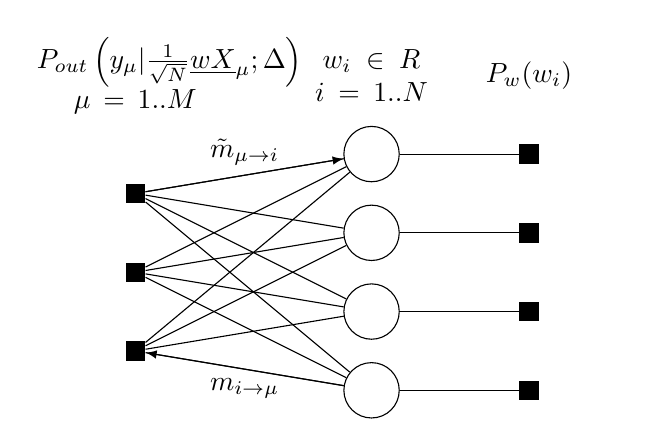
\begin{tikzpicture}
    \tikzstyle{factor}=[rectangle,fill=black,minimum size=7pt,inner sep=1pt]
    \tikzstyle{annot} = [text width=2.5cm, text centered]
       	
	\def\Nv{4}
	\def\Nu{3}
	\def\Nf{12}
	        
         \foreach \name / \y in {1,...,\Nu}
        \node[factor] (F2-\name) at (7,-0.5-\y) {};
        
        \foreach \name / \y in {1,...,\Nv}
        \node[latent] (W-\name) at (10,-\y) {};
        \foreach \name / \y in {1,...,\Nv}
        \node[factor] (PW-\name) at (12,-\y) {};
     	
%\edge {V-1}{F-1};

\path[-latex] (F2-1) edge node[above]{$\td{m}_{\mu \to i}$} (W-1);
\path[-latex] (W-4) edge node[below]{$m_{i \to \mu}$} (F2-3);

    \foreach \i in {1,...,\Nu}
    	 \foreach \j in {1,...,\Nv}
        	\edge[-]{F2-\i}{W-\j};  
        	
    \foreach \j in {1,...,\Nv}
    	\edge[-]{PW-\j}{W-\j};    	

\node[annot,above of=F2-1, node distance=1.5cm] {$P_{out}\(y_{\mu}|\frac{1}{\sqrt{N}}\ud{w}\ud{X}_{\mu};\Delta\)$ \\ $\mu =1 .. M$};
\node[annot,above of=W-1, node distance=1cm] (hl) {$w_i \in \mathbbm{R}$ \\ $i=1..N$};

\node[annot,above of=PW-1, node distance=1cm] {$P_w(w_i)$}; 

	\end{tikzpicture}
	\caption{Factor graph for $ M=3$, $N=4$}
	\label{factor_graph}
\end{figure}


\issue{\begin{itemize}
	\item The distribution $P\(\ud{w}| \ud{y}; \du{X}\)$ is intractable in the limit $N \to \infty$
	\item Hard to sample efficiently
\end{itemize}
}

\solution{Instead,
\begin{itemize}
	\item We may focus only on marginals $P(w_i;\ud{y},\du{X})$ which can been estimated with Belief Propagation (BP) equations and Approximate Message Passing (AMP) algorithms: See Part.\ref{AMP}
	\item We may also try to compute directly the free entropy $\Phi = \EE_{\ud{y},\ud{w}^0,\du{X}} \[\log\( \mZ\(\ud{y};\du{X} \) \) \]  $ with the replica method: See Part.\ref{Replicas}
	\item We try to give an idea how these two methods relate and we show they are complementary and consistent.
\end{itemize}
}

\newpage
\section{\Large Approximate Message Passing algorithm}

As we stressed above, the aim is to estimate the marginal probabilities $P(w_i;\ud{y},\du{X})$. We present a short overview how to derive the AMP algorithm, all the computation details are left in appendix.\\ 
The idea is to iterate partial "beliefs" between nodes of the graph until convergence towards the true marginal (if it converges).

\label{AMP}
\subsection{Step1: Belief Propagation (BP) equations}
Consider the factor graph \ref{factor_graph}.  
The first step is to write down the belief propagation equations. To do so, we imagine some \textit{messages/beliefs} $m_{i\to \mu}^{t+1} (w_i)$ and $\tilde{m}_{\mu \to i}^t (w_i) $, that we add on the edges of the factor graph. $t$ denotes the time of the iterations. Each message is the marginal probability of the variable $w_i$ if the edge between variable $i$ and constraint $\mu$ has been removed. BP equations read as follows: \\

\begin{equation}
	\begin{cases}
		m_{i\to \mu}^{t+1} (w_i) = \displaystyle \frac{1}{\mathcal{Z}_{i\to \mu}} P_0 (w_i) \prod\limits_{k \neq \mu}^M \tilde{m}_{\nu \to i}^t (w_i) \vspace{0.1cm}\\
		\tilde{m}_{\mu \to i}^t (w_i) =  \displaystyle \frac{1}{\mathcal{Z}_{\mu \to i}} \int \prod\limits_{j\neq i}^N dw_j P_{\rm out}\left (y_{\mu} | \displaystyle  \frac{1}{\sqrt{N}} \sum_{j=1}^N  X_{\mu j}w_{j} \right)  m_{j \to \mu}^t (w_j )\,,
	\end{cases}
	\label{supp:BPEquations}
\end{equation}
where BP equations assume that incoming messages are independent. Hence these equations are exact on a tree (no loop), but they remain exact if "correlations decrease fast enough / long loops". We assume in the following that the hypothesis is true in our model.\\

The idea is to expand in the limit $N \to \infty$ the message $\td{m}$ before plugging it in $m$. Keeping only terms of order $\mO\(1/N\)$ (See \ref{appendix:towardsrBP}), messages become \textit{Gaussian}. Hence we will be able to close the equations over only the mean and variance of the marginal distribution. Thus, we define the estimated mean and variance at time $t$ of the variable $j$ marginal probability.
\begin{equation*}
	\begin{cases}
		\hat{w}_{j\to \mu}^t \equiv\displaystyle \int_{\bbR} dw_j
		 m_{j\to \mu}^t (w_j ) w_j  \spacecase
		 \hat{c}_{j\to \mu}^t \equiv \displaystyle \int_{\bbR} dw_j
		 m_{j\to \mu}^t (w_j ) w_j w_j^\intercal - \hat{w}_{j\to \mu}^t(\hat{w}_{j\to \mu}^t)^\intercal
	\end{cases}
\label{What_Chat}
\end{equation*}


\subsection{Step 2: Towards relaxed BP}

The idea is to close equations over mean and variance $\hat{w}_{j\to \mu}^t$ and $\hat{c}_{j\to \mu}^t$ using:
\begin{enumerate}
	\item Fourier transform to decouple variables
	\item $N \to \infty$ expansion, keeping terms of order $\mO\(1/N\)$
\end{enumerate}

We show the derivation in \ref{appendix:towardsrBP}. In the end we obtain a set of $\mO(N^2)$ messages, called Relaxed BP equations:

\subsection*{Summary of the Relaxed BP set of equations}
In the end, Relaxed BP equations are simply the following set of equations:\\
\begin{minipage}[c]{.46\linewidth}
\begin{equation}
	\begin{cases}
	\hat{w}_{i\to \mu}^{t+1} = f_1^w(T_{\mu \to i}^t,\Sigma_{\mu \to i}^t ) \vspace{0.2cm} \\
	\hat{c}_{i \to \mu}^{t+1} = f_2^w(T_{\mu \to i}^t, \Sigma_{\mu \to i}^t) \vspace{0.2cm} \\
	\Sigma_{\mu \to i}^t = \left( \sum\limits_{\nu \ne \mu}^M  A_{\nu \to i}^t \right )^{-1} \vspace{0.2cm} \\
	T_{\mu \to i}^t = \Sigma_{\mu \to i}^t  \left( \sum\limits_{\nu \ne \mu}^M  B_{\nu \to i}^t \right)\vspace{0.2cm} \\
	\end{cases}
\end{equation}
\end{minipage}
 \hfill
\begin{minipage}[c]{.46\linewidth}
\begin{equation}
	\begin{cases}
			B_{\mu \to i}^t =  \frac{X_{\mu i}}{\sqrt{N}} g_{\rm out} (\omega_{i\mu}^t, y_{\mu}, V_{i\mu}^t)\vspace{0.2cm}  \\
		A_{\mu \to i}^t = - \frac{X_{\mu i}^2}{N}  \partial_\omega g_{\rm out}(\omega_{i\mu}^t, y_{\mu}, V_{i\mu}^t)\vspace{0.2cm} \\
		\omega_{i\mu}^t = \sum\limits_{j\neq i}^N \frac{X_{\mu j}}{\sqrt{N}}   \hat{w}_{j\to \mu}^t\vspace{0.2cm} \\
		V_{i\mu}^t = \sum\limits_{j\neq i}^N \frac{X_{\mu j}^2}{N} \hat{c}_{j\to \mu}^t \vspace{0.2cm}
	\end{cases}\\
	\label{supp:relaxed_BP}
\end{equation}      
\end{minipage}


where $f_1^w$ and $f_2^w$ are defined in \ref{update_functions}.


\subsection{Step 3: Towards Approximate Message Passing algorithm}
The relaxed BP algorithm uses $\mathcal{O}(N^2)$ messages. However all the messages depend weakly on the target node. The missing message is negligible in the limit $N \to \infty$, that allows us to expand the previous Relaxed BP equations \Eq{\ref{supp:relaxed_BP}}.\\

We define the "full" messages, where we removed the target node dependence:\\
\begin{minipage}[c]{.46\linewidth}
\begin{equation*}
	\begin{cases}
		\omega_{\mu}^t \equiv \sum\limits_{j = 1}^N \frac{X_{\mu j}}{\sqrt{N}}   \hat{w}_{j\to \mu}^t\vspace{0.1cm} \\
		V_{\mu}^t \equiv  \sum\limits_{j=1}^N \frac{X_{\mu j}^2}{N}   \hat{c}_{j\to \mu}^t\vspace{0.1cm} \\
	\end{cases}
\end{equation*}
\end{minipage} \hfill
\begin{minipage}[c]{.46\linewidth}
\begin{equation}
	\begin{cases}
		\Sigma_{i  }^t \equiv  \left( \sum\limits_{\nu =1}^M  A_{\nu \to i}^t \right )^{-1} \vspace{0.1cm} \\
	T_{i }^t \equiv  \Sigma_{i}^t  \left( \sum\limits_{\nu =1}^M  B_{\nu \to i}^t \right)\vspace{0.1cm} \\
	\end{cases}
\end{equation}
\end{minipage}

Expanding \Eq{\ref{supp:relaxed_BP}} around the above "full" messages, we obtain a closed set of equations over only $\mO(N)$ variables, called Generalized Approximate Message Passing (GAMP). We present the derivation in \Eq{\ref{appendix:towardsAMP}}. Finally the algorithm can be written as follows:

\subsection*{Summary - AMP algorithm}

\begin{algorithm} 
\begin{algorithmic}
    \STATE {\bfseries Input:} vector $y \in \bbR^M$ and matrix $X\in \bbR^{M \times N}$:
    \STATE \emph{Initialize}: $\hat{w}_i$, $g_{\rm out,\mu}$ $\in \bbR$ and $\hat{c}_i$, $\partial_{\omega} g_{\rm out , \mu}$ $\in \bbR^+$ for $ 1 \leq i \leq N $ and $ 1 \leq \mu \leq M $ at $t=0$.
    \REPEAT   
    \STATE Update of the mean $\omega_{\mu} \in \bbR$ and covariance $V_{\mu}\in \bbR^+$: \spacecase
    \hspace{0.5cm} $\omega_{\mu}^t = \sum\limits_{i = 1}^N \big(\frac{X_{\mu
      i}}{\sqrt{N}}\hat{w}_{i}^t -    \frac{X_{\mu
      i}^2}{N}
    \left(\Sigma_{i}^{t-1}\right)^{-1}\hat{c}_{i}^t \Sigma_{i
    }^{t-1}g_{\rm out,\mu}^{t-1} \big)  $  \spacecase
    \hspace{0.5cm} $V_{\mu}^t = \sum\limits_{i=1}^N\frac{X_{\mu
      i}^2}{N} \hat{c}_{i}^t $\spacecase
    \STATE Update of $g_{\rm out, \mu} \in \bbR$ and $\partial_{\omega} g_{\rm out , \mu} \in \bbR^+$: \spacecase
    \hspace{0.5cm}$g_{\rm out, \mu}^t = g_{\rm out} (\omega_{\mu}^t , Y_{\mu}, V_{\mu}^t) $ \spacecase
     \hspace{0.5cm} $ \partial_{\omega} g_{\rm out, \mu}^t = \partial_{\omega}  g_{\rm out} (\omega_{\mu}^t , Y_{\mu}, V_{\mu}^t)  $ \spacecase
    \STATE Update of the mean $T_i \in \bbR$ and covariance $\Sigma_i \in \bbR^+$:\spacecase
    \hspace{0.5cm}$T_i^t = \Sigma_{i}^t \Big(  \sum\limits_{\mu =1}^M
      \frac{X_{\mu
      i}}{\sqrt{N}}g_{\rm out,\mu}^t  -\frac{X_{\mu
      i}^2}{N}  \partial_{\omega} g_{\rm out , \mu}^t \hat{w}_{i}^t \Big) $ \spacecase 
      \hspace{0.5cm} $  \Sigma_{i}^t = -\Big(\sum\limits_{\mu =1}^M \frac{X_{\mu
      i}^2}{N}  \partial_\omega g_{\rm out,\mu}^t \Big)^{-1} $\spacecase
    \STATE Update of the estimated marginals $\hat{w}_i \in \bbR$ and $\hat{c}_i \in \bbR^+$: \spacecase
   \hspace{0.5cm}$\hat{w}_i^{t+1} = f_1^w( T_i^t,  \Sigma_i^t  ) $\spacecase
   \hspace{0.5cm}$   \hat{c}_i^{t+1} = f_2^w(T_i^t,  \Sigma_i^t  )$\spacecase
    \STATE ${t} = {t} + 1$ 
    \UNTIL{Convergence on
    $\hat{w}$, $\hat{c}$.} 
    \STATE {\bfseries Output:}
    $\hat{w}$ and $\hat{c}$.
\end{algorithmic}
\end{algorithm}



\newpage
\subsection{Step 4: State evolution equations - AMP}
We define the overlap parameters at time $t$, $m^t$, $q^t$, $\sigma^t$ and $Q^0$. Especially $m^t$ measures respectively correlation between the estimate of the student and the planted solution of the teacher.
\begin{align}
	\begin{cases}
	m^t \equiv \displaystyle \frac{1}{N} \sum_{i=1}^N \hat{w}^t_i(w^0_i)^\intercal \\
	q^t \equiv \displaystyle \frac{1}{N} \sum_{i=1}^N \hat{w}^t_i(\hat{w}^{t}_i)^\intercal  
	\end{cases}
	\hspace{0.3cm} \textrm{ and } \hspace{0.3cm}
	\begin{cases}
	Q^0 \equiv \displaystyle \frac{1}{N} \sum_{i=1}^N w^0_i(w^0_i)^\intercal \\ 
	\sigma^t \equiv \displaystyle \frac{1}{N} \sum_{i=1}^N \hat{c}_{i}^{t} \\
	\end{cases}
	\label{amp_overlaps}
\end{align}
The aim is to derive the asymptotic state evolution equations of these overlap parameters, starting with the relaxed BP equations \Eq{\ref{supp:relaxed_BP}}. The idea is to compute the statistics of each variable to finally get the distribution of the above overlaps parameters.\\

The computation is shown in \ref{appendix:state_evolution_amp}.

\subsection{Conclusion - Bayes optimal case}
In the Bayes optimal case, the student knows the true prior, channel distribution and in particular using Nishimori identities:
\begin{align*}
	\begin{cases}
		P_{w^0} = P_w \spacecase
		P^0_{out} = P_{out} \spacecase
		m^t = q^t \spacecase
	\end{cases}
\end{align*}

In this case, the State Evolution (SE) equation read as scalar iterative equations:
\begin{align}
	\begin{cases}
		q^{t+1}  = \EE_{\xi} \[ \displaystyle f^w_0\( \lambda^t[ \xi ], \sigma^t \) f^{w}_1\( \lambda^t[ \xi ], \sigma^t \) f^{w}_1\( \lambda^t[ \xi ], \sigma^t \)^\intercal \] \spacecase 
		\hat{q}^t = \alpha  \EE_{y, \xi}\[ f_{out}(y, \omega^t[\xi] ,  V^t  ) g_{out}(y, \omega^t[\xi] ,  V^t  ) g_{out}(y, \omega^t[\xi] ,  V^t  ) \] \spacecase
	\end{cases}
	\andcase
		\begin{cases}
	\lambda^t[\xi] \equiv ( \hat{q}^t)^{-1/2}  \xi  \spacecase
	\sigma^t \equiv (\hat{q}^t)^{-1} \spacecase
	\omega^t[\xi] = (q^t)^{1/2} \xi\spacecase
	V^t = Q^0 - q^t
	\end{cases}
	\label{amp_state_evolution}
\end{align}

with $f_{out}, g_{out}$, $f_0^w$ and $f_1^w$ defined in \ref{update_functions}. The derivation is shown in \ref{appendix:state_evolution_amp} and \ref{appendix:state_evolution_amp_replicas}.\\

In the limit $N\to \infty$ the overlap of the algorithm is controlled by the above equations. However, the algorithm works at finite, but large, $N$ and its practical overlap fluctuates around the overlap given by the SE.\\
Besides, we will see in the next part that these equations can be interpreted as doing "gradient descent on the Replica Symmetric" potential. 

\subsection{Update functions}
\label{update_functions}
Where the update functions read:

\subparagraph{$f_0^w$}
\begin{equation}
	\begin{cases}
	\td{P}_w(w, \lambda,\sigma)\equiv \displaystyle \frac{1}{f_0^w (\lambda ,\sigma)} P_w(w) e^{ - \frac{1}{2} w\sigma^{-1} w  + \lambda \sigma^{-1}w  } \spacecase 
		f_0^w (\lambda ,\sigma) = \displaystyle \int_{\bbR^K} dw P_w(w) e^{ - \frac{1}{2} w\sigma^{-1} w  + \lambda \sigma^{-1}w  }
	\end{cases}
	\begin{cases}
		f_1^w(\lambda ,\sigma) = \EE_{\td{P}_w} \[ w \]\spacecase
		f_2^w (\lambda ,\sigma) =  \EE_{\td{P}_w} \[ w w \] - f_1^w (f_1^w) 
	\end{cases}
	\label{appendix:update_functions:f1_w-f2_w}
\end{equation}

\subparagraph{$f_{out}$}
\begin{equation}
	\begin{cases}
	\td{P}_{out} (z; y,\omega,V) = \frac{1}{f_{out}(y,\omega,V)} P_{out}\(y | \varphi_{out} \( z; \Delta \) \)  e^{ -\frac{1}{2} \(z - \omega\) V^{-1} \(z - \omega\) }\spacecase
		f_{out}(y,\omega,V)  = \mN(V) \displaystyle \int_{\bbR}  d z P_{out}\(y | \varphi_{out} \( z; \Delta \) \)  e^{ -\frac{1}{2} \(z - \omega\) V^{-1} \(z - \omega\) } \spacecase
			g_{out}(y,\omega,V) = \displaystyle \frac{1}{f_{out}} \frac{\partial f_{out}}{\partial \omega} = V^{-1} \mE_{\td{P}_{out}} \[ z - \omega\] \spacecase
		\partial_{\omega} g_{out} (y,\omega,V) = \displaystyle \frac{\partial g_{out}}{\partial \omega} = V^{-1} \mE_{\td{P}_{out}} \[ (z - \omega)(z - \omega)\]V^{-1} -V^{-1} - g_{out}^2(y,\omega,V)  \spacecase
	\end{cases}
	\label{appendix:update_functions:fout-gout}
\end{equation}






\newpage
\section{\Large Replicas computation}
\label{Replicas}
An other approach to tackle this high dimensional Bayesian inference is to compute the averaged free entropy $\Phi$. This is the central object of study in disordered systems and it can be computed using the replica method.\\

We will show that in fact state evolution of the AMP algorithm can be obtained directly from the replica free entropy saddle point.

\subsection{Step 1: Partition function and replica trick}
\subsubsection{Partition function, free entropy and average scenario}

Let's define the partition function $\mZ$ as the normalizing constant in \Eq{\ref{distribution_P}}, that reads integrating over $\ud{w}$:
\begin{align}
	\mZ\(\ud{y};\du{X}\) \equiv \mP\(\ud{y};\du{X}\)  = \int_{\bbR^{N}}  d\ud{w} P_w(\ud{w}) \int_{\bbR^{M}} d\ud{z} P_{out} \(\ud{y} | \varphi_{out}\( \ud{z},  \Delta\) \) \delta\(\ud{z}-\frac{1}{\sqrt{N}}
	\ud{w}\du{X}\) 
\end{align}

As we consider the average scenario, we need to average over the training set $\{\ud{y}, \du{X}\}$ and the planted solution $\ud{w}^0$. The averaged free entropy reads then:
\begin{align}
	\Phi &= \lim_{N \to \infty} \frac{1}{N} \EE_{\ud{y},\ud{w}^0,\du{X}} \[\log \Z(\ud{y};\du{X}) \]\\
	&= \displaystyle \lim_{N \to \infty} \EE_{\du{X}} \[\int_{\bbR^M} d\ud{y} \int_{\bbR^{N}}  d\ud{w}^0  P_{w^0}(\ud{w}^0) \int_{\bbR^{M}} d\ud{z}^0 P_{out}^0 \(\ud{y} | \varphi_{out}^0\( \ud{z}^0;\Delta^0 \) \)  \delta\(\ud{z}^0-\frac{1}{\sqrt{N}}
	\ud{w}^0\du{X}\)  \times ... \right. \\
	   & ... \left. \times  \log \( \int_{\bbR^{N}}  d\ud{w} P_w(\ud{w}) \int_{\bbR^{M}} d\ud{z} P_{out} \(\ud{y} | \varphi_{out}\( \ud{z},  ;\Delta\) \)  \delta\(\ud{z}-\frac{1}{\sqrt{N}}
	\ud{w}\du{X}\)  \)\]
\end{align}

\subsubsection{Replica trick}

This average of the logarithm is intractable. Instead we use the so-called \textit{Replica trick}: 
$\EE[\log(z)] = \lim_{n \to 0} \frac{1}{n} \log \EE[z^n]$. Applying it to the free entropy gives:
\begin{align}
	\Phi &= \lim_{N \to \infty} \EE_{\du{X}} \[ \phi\(\du{X}\)\] = \lim_{N \to \infty} \frac{1}{N} \EE_{\ud{y},\ud{w}^0,\du{X}} \[\log \Z(\ud{y};\du{X}) \] = \lim_{n \to 0} \frac{1}{Nn} \log \EE_{\ud{y},\ud{w}^0,\du{X}} \[ \Z(\ud{y};\du{X})^n \]
\end{align}

\subsection{Step 2: Average over disorder and interacting copies}

\paragraph{Average of the moments}
Remains to compute the averaged $n$-th moment of the partition function: $\EE_{\ud{y},\ud{w}^0,\du{X}} \[ \Z(\ud{y};\du{X})^n \]$. Note that computing $\mZ^n$ for $n \in \bbN$ corresponds to compute the partition function of $n$ non-interacting copies of the same system.

\begin{align}
	\EE_{\ud{y},\ud{w}^0,\du{X}} \[ \Z(\ud{y};\du{X})^n \] &= \EE_{\du{X}} \[ \int_{\bbR^{M}}d\ud{y}  \int_{\bbR^{N}} d\ud{w}^0 P_{w^0}(\ud{w}^0)   \int_{\bbR^{M}}d\ud{z}^0  P_{out}^0\(\ud{y} | \varphi_{out}^0\(\ud{z}^0;\Delta^0\)\) \delta(\ud{z}^0-\frac{1}{\sqrt{N}}\du{X}\ud{w}^0 ) \right. \\ 
	& \left. \prod_{a=1}^n \int_{\bbR^{N}} d\ud{w}^a P_{w^a}(\ud{w}^a) \int_{\bbR^{M}}d\ud{z}^a  P_{out}\(\ud{y} | \varphi_{out}\(\ud{z}^a; \Delta  \)\) \delta(\ud{z}^a-\frac{1}{\sqrt{N}}\du{X}\ud{w}^a ) \]\\
	&= \EE_{\du{X}} \[  \prod_{a=0}^n \int_{\bbR^{N}} d\ud{w}^a P_{w^a}(\ud{w}^a) \int_{\bbR^{M}}d\ud{z}^a  P_{out}^a\(\ud{y} | \varphi_{out}^a\(\ud{z}^a; \Delta^0  \)\) \delta(\ud{z}^a-\frac{1}{\sqrt{N}}\du{X}\ud{w}^a ) \]
\end{align}

where we consider the teacher solution as an other replica with index $a=0$. Note that\\ 
$$P_{w^a} = \begin{cases}
	P_{w^0} \textrm{ if } a=0 \\
	P_{w} \textrm{ if } a\ne 0 \\
\end{cases}, P_{out}^a = \begin{cases}
	P_{out}^0 \textrm{ if } a=0 \\
	P_{out} \textrm{ if } a\ne 0 \\
\end{cases} \varphi_{out}^a = \begin{cases}
	\varphi_{out}^0 \textrm{ if } a=0 \\
	\varphi_{out} \textrm{ if } a\ne 0 \\
\end{cases}
\andcase  \Delta^a = \begin{cases}
	\Delta^0 \textrm{ if } a=0 \\
	\Delta \textrm{ if } a\ne 0 \\
\end{cases}$$

\paragraph{Average over $X$}
The first step is to take advantage of the $iid$ property of the disorder distribution $P_x \sim \mN(0,1)$.\\

Let's consider the variable $z^a_{\mu} = \displaystyle \frac{1}{\sqrt{N}}\sum_{i=1}^N  X_{\mu i} w_{i}^a $. Using CLT, the vector $z^a_{\mu}$ follows a multivariate gaussian distribution such that: 
\begin{align}
		\EE_{\du{X}} \[ z^a_{\mu} \] = 0 \hspace{0.3cm} \textrm{ and } \hspace{0.3cm}
		\EE_{\du{X}} \[ z^a_{\mu}z^b_{\nu} \] = \frac{1}{N} \sum_{i=1}^N w_{i}^a w_{i}^b  \delta_{\mu \nu}
\end{align}

\solution{
\begin{enumerate}
	\item Replicas were identical and non-interacting as it was the copy of $n$ identical systems. Strikingly, averaging over the disorder makes replicas interact!
	\item Besides it naturally introduces the order parameter, called the \textit{overlap} $Q_{ab} = \frac{1}{N} (\ud{w}^a)^\intercal\ud{w}^b $, that measures the correlation between replicas.
\end{enumerate} }

From the above average, $\ud{\tbf{z}}$ follows a  multivariate distribution of size $ M \times (n+1)$: $P_z(\ud{\tbf{z}}) = \frac{e^{-\frac{1}{2}\ud{\tbf{z}}^\intercal \du{\boldsymbol{\Sigma}}^{-1} \ud{\tbf{z}} }}{(2\pi)^{M (n+1)/2}  \det(\du{\boldsymbol{\Sigma}})^{M/2}} $, with the matrix of overlaps as covariance matrix:
\begin{align}
	\(\du{\boldsymbol{\Sigma}}\)_{ab} = Q_{ab} \equiv \frac{1}{N} \sum_{i=1}^N w_{i}^a w_{i}^b = \frac{1}{N} (\ud{w}^a)^\intercal\ud{w}^b
\end{align}

The overlap being the natural order parameter, we introduce the change of variable multiplying by $$\displaystyle 1 = \int \prod_{(a,b)} dQ_{ab} \delta\(N Q_{ab} - \sum_{i=1}^N w_{i}^a w_{i}^b\) $$.

\begin{align}
	&\EE_{\ud{y},\ud{w}^0,\du{X}} \[ \Z(\ud{y};\du{X})^n \] = \int_{\bbR^{(n+1)\times(n+1)}} \prod_{(a,b)} dQ_{ab} \\
	&  \int d\ud{y}     \int_{\bbR^{M\times (n+1)}} \prod_{a=0}^n d\ud{z}^a  P_{out}^a\(\ud{y} | \varphi_{out}^a\(\ud{z}^a;\Delta^a\)\) \exp\(-\frac{1}{2} \sum_{\mu=1}^M \sum_{ab} z^a_{\mu }z^b_{\mu} (\Sigma_{ab})^{-1}  - \frac{M}{2}\log(\det{\du{\boldsymbol{\Sigma}}}) - \frac{M(n+1)}{2}\log(2\pi) \) \\
	&  \int \prod_{a=0}^n d\ud{w}^a P_{w^a}(\ud{w}^a) \prod_{(a,b)} \delta\(N Q_{ab} - \sum_{i=1}^N w_{i}^a w_{i}^b\)
\end{align}

%Next we introduce the Fourier representation of the Dirac function involved in the change of variable. It finally decouples the directions $\mu$ and $i$ (because $P_w$ and $P_{out}$ decouple along one direction).

Next we introduce the Fourier representation of the Dirac function to factorize the integral: $$\displaystyle \delta\(N Q_{ab} - \sum_{i=1}^N w_{i}^a w_{i}^b\) = \int d \hat{Q}_{ab} e^{\hat{Q}_{ab} \(N Q_{ab} - \sum_{i=1}^N w_{i}^a w_{i}^b \)}$$. As $P_w$ and $P_{out}$ factorize, it allows to decouple the replicated partition functions as  \textit{prior} and \textit{channel} terms: 

\begin{align}
	&\EE_{\ud{y},\ud{w}^0,\du{X}} \[ \Z(\ud{y};\du{X})^n \] =\int_{\bbR^{(n+1)\times(n+1)}} \prod_{(a,b)} dQ_{ab} \int_{\bbR^{(n+1)\times(n+1)}} \prod_{(a,b)} d\hat{Q}_{ab}  \prod_{(a,b)}\exp \(N\hat{Q}_{ab}  Q_{ab}\) \\
	&  \int_{\bbR^M} d\ud{y}    \int_{\bbR^{M\times (n+1)}} \prod_{a=0}^n d\ud{z}^a  P_{out}^a\(\ud{y} | \varphi_{out}^a\(\ud{z}^a;\Delta^a\)\) \exp\(-\frac{1}{2} \sum_{\mu=1}^M \sum_{ab} z^a_{\mu}z^b_{\mu} (\Sigma_{ab})^{-1}  - \frac{M}{2}\log(\det{\du{\boldsymbol{\Sigma}}}) - \frac{M(n+1)}{2}\log(2\pi) \) \\
	& \int_{\bbR^{N\times (n+1)}} \prod_{a=0}^n d\ud{w}^a P_{w^a}(\ud{w}^a) \prod_{(a,b)}\exp \(- \hat{Q}_{ab}\sum_{i=1}^N w_{i}^a w_{i}^b\)\\
	&=\int_{\bbR^{(n+1)\times(n+1)}} \prod_{(a,b)} dQ_{ab} \int_{\bbR^{(n+1)\times(n+1)}} \prod_{(a,b)} d\hat{Q}_{ab}  \prod_{(a,b)}\exp \(N\hat{Q}_{ab}  Q_{ab}\) \\
	&  \[ \int_{\bbR} dy   \int_{\bbR^{n+1}} \prod_{a=0}^n dz^a  P_{out}^a\(y | \varphi_{out}^a\(z^a;\Delta^a\)\) \exp\(-\frac{1}{2} \sum_{ab} z^a z^b (\Sigma_{ab})^{-1}  - \frac{1}{2}\log(\det{\du{\boldsymbol{\Sigma}}}) - \frac{(n+1)}{2}\log(2\pi) \)\]^M \\
	& \[ \int_{\bbR^{n+1}} \prod_{a=0}^n dw^a P_{w^a}(w^a) \prod_{(a,b)}\exp \(- \hat{Q}_{ab} w^a w^b\)\]^N
\end{align}


\paragraph{Conclusion}
To conclude we need to use "non rigorous" tricks:
\begin{enumerate}
	\item use an analytic continuation for $n\in \bbN$ that becomes $n \in \bbR$, before taking the limit $n\to0$
	\item exchange the limits $N \to \infty$ and $n \to 0$...
	\item use a Laplace method of the integrals in the $N \to \infty$ limit
\end{enumerate}


Doing so, the free entropy reads as a saddle point:
\begin{align}
	\Phi = &\frac{1}{N} \EE_{\ud{y},\ud{w}^0,\du{X}} \[\log \Z(\ud{y};\du{X}) \] = \lim_{n \to 0} \frac{1}{Nn} \log \EE_{\ud{y},\ud{w}^0,\du{X}} \[ \Z(\ud{y},\du{X})^n \]\\
	&= \lim_{n \to 0} \frac{1}{n} \extr_{\du{\tbf{Q}},\du{\hat{\tbf{Q}}}} \left \{\mH(\du{\tbf{Q}},\du{\hat{\tbf{Q}}} ) \right\}
\end{align}

where:
\begin{align}
	\begin{cases}
	\mH(\du{\tbf{Q}},\du{\hat{\tbf{Q}}} ) &\equiv \sum_{ab} \hat{Q}_{ab}  Q_{ab} + \log\(\hat{\mI}_w(\du{\hat{\tbf{Q}}})\) + \alpha \log\(\hat{\mI}_z(\du{\tbf{Q}};\Delta\)  \spacecase
		\hat{\mI}_w(\du{\hat{\tbf{Q}}}) &\equiv \displaystyle  \int_{\bbR^{n+1}} \prod_{a=0}^n dw^a P_{w^a}(w^a) \prod_{(a,b)}\exp \(- \hat{Q}_{ab} w^a w^b\) \spacecase 
		\hat{\mI}_z(\du{\tbf{Q}};\Delta) &\equiv \displaystyle \int_\bbR d y     \int_{\bbR^{n+1}}  \prod_{a=0}^n dz^a  P_{out}^a\(y | \varphi_{out}^a\(z^a;\Delta\)\) \times \exp\(-\frac{1}{2} \sum_{ab} z^a z^b (\Sigma^{ab})^{-1}  - \frac{1}{2}\log(\det{\du{\boldsymbol{\Sigma}}}) - \frac{(n+1)}{2}\log(2\pi) \)
	\end{cases}
\end{align}

Computing the free entropy is reduced to an optimization problem over two matrices $\du{\tbf{Q}},\du{\hat{\tbf{Q}}} \in \bbR^{(n+1)\times (n+1)}$.

\newpage
\subsection{Step 3: RS assumption}
To take the limit $n \to 0$, we need an analytical expression for the potential $\mH(\du{\tbf{Q}},\du{\hat{\tbf{Q}}} )$ as a function of $n$.\\
Hence we assume a simple ansatz saying that the critical point of $\mH$ is reached for a value $\du{\tbf{Q}}^w$ and $\du{\hat{\tbf{Q}}}^w$ which verify the Replica Symmetric assumption. More precisely, matrices $\du{\tbf{Q}},\du{\hat{\tbf{Q}}}$ verify:
\begin{equation}
	\du{\tbf{Q}}^w=\begin{bmatrix}
    Q^0 & m & m & m  \\
    m & Q & q & q \\
    m & q & Q & q \\
    m & q & q & Q \\
  \end{bmatrix}
  \hspace{1cm}
  \du{\hat{\tbf{Q}}}^w=\begin{bmatrix}
    \hat{Q}^0 & \hat{m} & \hat{m} & \hat{m}  \\
    \hat{m} & \hat{Q} & \hat{q} & \hat{q} \\
    \hat{m} & \hat{q} & \hat{Q} & \hat{q} \\
    \hat{m} & \hat{q} & \hat{q} & \hat{Q} \\
  \end{bmatrix}
\end{equation}

Note that we recover naturally the overlaps defined in AMP \Eq{\ref{amp_overlaps}}. These quantities have strong interpretation: $m$ measures the correlation between the estimator and the planted solution, $q$ is the correlation between different replicas, and $Q, Q^0$ are the norms of replicas and planted solutions. As showed above, the variable $\du{\hat{Q}}$ has no physical meaning as it has been introduced with the Fourier representation of the Dirac function. Besides the RS assumption means that we assume that correlations between replicas (except the one corresponding to the teacher) are the same, meaning they belong to a same "state" or "cluster" of solution.  \\

\begin{align}
	\begin{cases}
		m = \frac{1}{N} (\ud{w}^0)^\intercal \ud{w}^a \textrm{ for $a\ne 0$} \spacecase
		q = \frac{1}{N} (\ud{w}^a)^\intercal \ud{w}^b \textrm{ for $a\ne b$} \spacecase
	\end{cases}
	\andcase
	\begin{cases}
		Q^0 = \frac{1}{N} (\ud{w}^0)^\intercal \ud{w}^0 \spacecase
		Q = \frac{1}{N} (\ud{w}^a)^\intercal \ud{w}^a \textrm{ for $a\ne 0$}  \spacecase
	\end{cases}
\end{align}

\issue{Note that in general the RS assumption is wrong. To check this, we need to study its stability (computing the eigenvalues of the hessian). It leads to Replica Symmetry Breaking (RSB). However in the Bayes optimal case, the RS ansatz is correct. \\}

Using this simple RS ansatz, we can now explicit the replica potential: 
\begin{align}
	\mH(\du{\tbf{Q}},\du{\hat{\tbf{Q}}} ) &\equiv \sum_{ab} \hat{Q}_{ab}  Q_{ab} + \log\(\hat{\mI}_w(\du{\hat{\tbf{Q}}})\) + \alpha \log\(\hat{\mI}_z(\du{\tbf{Q}};\Delta\)
\end{align}

We show details of the computation in \Eq{\ref{appendix:rs_assumption}}. In the end we obtain an expression that is explicit in $n$:
 \begin{align}
 	\begin{cases}
 		&\hat{\mI}_w(\du{\hat{\tbf{Q}}}) = \displaystyle  \int_{\bbR} D\xi  \int_{\bbR}  d w^0 P_{w^0}(w^0) e^{-(w^0)^\intercal \hat{Q}^0_w w^0}  \[ \int_{\bbR}  d w P_w(w) \exp \( - \[ 2 w^0 \hat{m} w + w \( \hat{Q} + \hat{q}\) w - \xi \hat{q}^{1/2} w  \] \) \]^n \spacecase
 		&\hat{\mI}_z(\du{\tbf{Q}};\Delta) = \displaystyle \int D \xi \int dy  \e^{\displaystyle - \frac{1}{2}\log(\det{\du{\boldsymbol{\Sigma}}}) - \frac{(n+1)}{2}\log(2\pi) }  \int d z^0  P_{out}^0\(y | \varphi_{out}^0\(z^0; \Delta^0 \)\) e^{\displaystyle -\frac{1}{2}\( z^0 \Sigma^{-1}_{00} z^0  \)  } \\
	& \[ \int dz  P_{out}\(y | \varphi_{out}\( z; \Delta \)\) e^{\displaystyle - z^0 \Sigma^{-1}_{01} z -\frac{1}{2}  z \( \Sigma^{-1}_{11} - \Sigma^{-1}_{12} \)z  - \xi \Sigma^{-1/2}_{12} z } \]^n
 	\end{cases}
 \end{align}



\paragraph{ Check $n \to 0$ limit}
We need to check that $ \lim_{n \to 0} \extr_{\du{\tbf{Q}},\du{\hat{\tbf{Q}}}} \left \{\mH(\du{\tbf{Q}},\du{\hat{\tbf{Q}}} ) \right\} \longrightarrow 0 $. Doing so leads to  (\Eq{\ref{appendix:check_n_0}}): 
\begin{align*}
	\begin{cases}
		\hat{Q}^0 = 0 \spacecase
		Q^0 = \EE_{P_{w^0}} \[w^0 w^0 \]
	\end{cases}
\end{align*}


\subsection{Step 4: $n \to 0$ limit}

The last step consists in dividing by $n$ and taking the $n \to 0$ limit.\\

\solution{\begin{itemize}
	\item Note that we exchanged the order of the limit $N \to \infty$ and $n \to 0$: we use the Laplace method before taking $n \to 0$
	\item The computation is long, painful and does not give any insights. We skip the details and we refer to \Eq{\ref{appendix:check_limit_n_0}}  
	\item However, in a few words the idea is to decouple interacting replicas using a Hubbard-Stratanovich / Gaussian transformation : $\int  \frac{e^{- \frac{y^2}{2 a} }}{\sqrt{2\pi a}} e^{xy} dy= e^{-a x^2/2}$
\end{itemize}}

\begin{align}
	\Phi &= \lim_{n \to 0} \frac{1}{n} \extr_{\du{\tbf{Q}},\du{\hat{\tbf{Q}}}} \left \{\mH(\du{\tbf{Q}},\du{\hat{\tbf{Q}}} ) \right\}
\end{align}

\subsection{Conclusion - Bayes optimal case}
In the Bayes optimal setting, using Nishimori Identities,

\begin{align*}
	\begin{cases}
		Q = Q^0 = \EE_{P_w^0}\[w^0 w^0 \] \spacecase
		\hat{Q} = \hat{Q}^0 = 0 \spacecase
	\end{cases}
	\andcase
	\begin{cases}
		q = m \spacecase
		\hat{q} = \hat{m} \spacecase
  	\end{cases}
  	\andcase
  	\begin{cases}
  		P_{w^0}= P_w \spacecase
  		P_{out}^0 = P_{out} \spacecase
  	\end{cases}\, ,
\end{align*} 
the Replica Symmetric (RS) free entropy (See \ref{appendix:RS_free_entropy}) simplifies and reads as an optimization problem over two scalar parameters $q$ and $\hat{q}$:

\begin{align}
		\Phi = &\frac{1}{N} \EE_{\ud{y},\ud{w}^0,\du{X}} \[\log \Z(\ud{y};\du{X}) \] =\extr_{q,\hat{q}}\left \{ -\frac{1}{2} q \hat{q}  +  \mI_w\(\hat{q}  \) + \alpha \mI_z\(Q^0, q; \Delta\) \right\} 
	\label{main:conclusion_second_layer_non_bayes}
\end{align}
where
\begin{align}
\begin{cases}
		  \mI_z\(Q^0, q; \Delta\) = \EE_{y, \xi } \[ f_{out}\(y,\omega[\xi]  , V ; \Delta  \) \log f_{out}\(y,\omega[\xi]  , V ; \Delta \)  \] \spacecase
		\mI_w\(\hat{q}\) =  \EE_{\xi } \[ f_0^w\( \lambda[\xi]  , \sigma  \) \log f_0^w\(\lambda[\xi]  , \sigma  \)   \]
\end{cases}
\andcase
\begin{cases}
	\sigma^{-1}\lambda[\xi]  = \hat{q}^{1/2}\xi   \spacecase
	\sigma = \( \hat{q}\)^{-1}\spacecase
	\omega[\xi] = q^{1/2}\xi\spacecase
	V = \(Q^0- q \) \spacecase
\end{cases}
\end{align}

with $f_{out}$ and $f_0^w$ defined in \Eq{\ref{update_functions}}

\solution{\begin{itemize}
\item 	To legitimate all non rigorous tricks we used, it is worth noting that this free entropy can be proved rigorously. However, usually the proof requires the replica free entropy expression...!
\item See \cite{Bayati}, \cite{Rangan}, \cite{Barbier2017b}.
\end{itemize}
}



\subsection{State evolution and consistence with replicas}

Taking the saddle point of \Eq{\ref{main:conclusion_second_layer_non_bayes}}, and using integration by part, we obtain: 


\begin{align*}
	\begin{cases}
		q  = \EE_{\xi} \[ \displaystyle f^w_0\( \lambda[ \xi ], \sigma \) f^{w}_1\( \lambda[ \xi ], \sigma \) f^{w}_1\( \lambda[ \xi ], \sigma \) \] \spacecase
		\hat{q} = \alpha  \EE_{y, \xi}\[ f_{out}(y, \omega[\xi] ,  V  ) g_{out}(y, \omega[\xi] ,  V  ) g_{out}(y, \omega[\xi] ,  V  ) \] \spacecase
	\end{cases}
\end{align*}


This formulation is equivalent to the one we obtain with AMP\Eq{\ref{amp_state_evolution}}, except we do not have the time indices... !\\
Hence the state evolution of the AMP algorithm does a gradient descent of the RS free entropy (in the Bayes optimal case). 







\newpage
\section{\Large References}
\bibliography{library,lib,lib2}



\newpage
\section{\Large Appendices}


\subsection{Towards relaxed BP}
\label{appendix:towardsrBP}
The term inside $P_{\rm out}$ can be decoupled using its Fourier transform:
\begin{equation*}
P_{\rm out}\left (y_{\mu} | \displaystyle \frac{1}{\sqrt{N}} \sum_{j=1}^N  X_{\mu j}w_{j} \right) = \frac{1}{(2\pi)^{K/2}}
\int_{\bbR} d \xi \exp\left( i \xi^\intercal \left( \displaystyle \frac{1}{\sqrt{N}} \sum_{j=1}^N  X_{\mu j}w_{j}\right) \hat{P}_{\rm out}(y_{\mu} , \xi )    \right).	
\end{equation*}
Injecting this representation in the BP equations, \eqref{supp:BPEquations} becomes:
\begin{align*}
&\tilde{m}_{\mu \to i}^t (w_i ) = 
\frac{1}{(2\pi)^{K/2}\mathcal{Z}_{\mu\to i} }
\int_{\bbR} d\xi \hat{P}_{\rm out}(y_{\mu} , \xi)  
\exp\left(i  \xi^\intercal \frac{1}{\sqrt{N}} X_{\mu i} w_i \right)\nonumber\\
 &\qquad\qquad\qquad\qquad\times\prod\limits_{j\neq i}^N  \underbrace{\int_{\bbR} dw_j 
		 m_{j \to \mu}^t (w_j ) \exp\left( i  \xi^\intercal \frac{1}{\sqrt{N}} X_{\mu j} w_j ) \right)}_{\equiv I_j}
		 \label{mtilde}
\end{align*}

In the limit $n\to \infty$ the term $I_j$ can be easily expanded and expressed using $\hat{w}$ and $\hat{c}$:
\begin{align*}
 I_j &= \int_{\bbR} dw_j
		 m_{j \to \mu}^t (w_j ) \exp\left( i  \xi^\intercal \frac{X_{\mu j}}{\sqrt{N}} w_j ) \right) \simeq  \exp\left( i \frac{X_{\mu j}}{\sqrt{N}}\xi^\intercal  \hat{w}_{j\to \mu}^t -  \frac{1}{2}\frac{X_{\mu j}^2}{N} \xi^\intercal  \hat{c}_{j\to \mu}^t  \xi\right) .
\end{align*} 

And finally using the inverse Fourier transform:
\begin{align*}
&\tilde{m}_{\mu \to i}^t (w_i ) = 
\frac{1}{(2\pi)\mathcal{Z}_{\mu \to i}}
\int_{\bbR} dz P_{\rm out}(y_\mu , z ) 
\int_{\bbR} d \xi  
e^{-i \xi^\intercal z}
e^{ i X_{\mu i} \xi^\intercal w_i} \\
&\qquad\qquad\qquad\qquad\qquad\times\prod\limits_{j\neq i}^N  \exp\left( i \frac{X_{\mu j}}{\sqrt{N}} \xi^\intercal \hat{w}_{j\to \mu}^t -  \frac{1}{2}\frac{X_{\mu j}^2}{N} \xi^\intercal \hat{c}_{j\to \mu}^t \xi\right) \\
&= \frac{1}{(2\pi)\mathcal{Z}_{\mu\to i}}
\int_{\bbR} dz
P_{\rm out}(y_\mu , z )
\int_{\bbR} d \xi  
e^{-i \xi^\intercal z}
e^{ i X_{\mu i} \xi^\intercal w_i} e^{i \xi^\intercal \sum\limits_{j\neq i}^N \frac{X_{\mu j}}{\sqrt{N}} \hat{w}_{j\to \mu}^t } e^{-  \frac{1}{2} \xi^\intercal \sum\limits_{j\neq i}^N \frac{X_{\mu j}^2}{N}   \hat{c}_{j \to \mu }^t\xi} \\
&= \frac{1}{(2\pi)\mathcal{Z}_{\mu\to i}} \int_{\bbR} dzP_{\rm out}(y_\mu , z)\sqrt{\frac{(2\pi)}{\det(V_{i \mu }^t)}} \underbrace{e^{-\frac{1}{2} \left( z -\frac{X_{\mu i}}{\sqrt{N}} w_i -\omega_{i \mu}^t \right)^\intercal (V_{i \mu }^t)^{-1} \left( z -\frac{X_{\mu i}}{\sqrt{N}} w_i -\omega_{i \mu}^t \right)}}_{\equiv H_{i\mu}}
\end{align*}
where we defined the mean and variance, depending on the node $i$:
\begin{equation*}
	\begin{cases}
	\omega_{i \mu}^t \equiv  \frac{1}{\sqrt{N}} \sum\limits_{j\neq i}^N X_{\mu j}  \hat{w}_{j\to \mu}^t \\
		V_{i\mu}^t \equiv  \frac{1}{N} \sum\limits_{j\neq i}^N X_{\mu j}^2  \hat{c}_{j \to \mu}^t
	\end{cases}
\end{equation*}


Again, in the limit $n\to \infty$, the term $H_{i\mu}$ can be expanded:
\begin{align*}
	H_{i\mu} &\simeq   e^{-\frac{1}{2} \left( z -\omega_{i \mu}^t \right)^\intercal (V_{i\mu}^t)^{-1} \left( z -\omega_{i \mu}^t \right) } 
	\left( 1 + \frac{X_{\mu i}}{\sqrt{N}} w_i^\intercal (V_{i\mu}^t)^{-1} (z -\omega_{i \mu}^t) -\frac{1}{2}\frac{X_{\mu i}^2}{N} w_i^\intercal (V_{i\mu}^t)^{-1} w_i \right.\\
& \left. + \frac{1}{2} \frac{X_{\mu i}^2}{N} w_i^\intercal (V_{i\mu}^t)^{-1} (z -\omega_{i \mu}^t)(z -\omega_{i \mu}^t)^\intercal  (V_{i\mu}^t)^{-1} w_i \right).
\end{align*}
Gathering all pieces, the message $\tilde{m}_{\mu \to i}$ can be expressed using definitions of $g_{\rm out}$ and $\partial_{\omega} g_{\rm out}$:

\begin{align*}
\tilde{m}_{\mu  \to i}^t (w_i ) &\sim \frac{1}{\mathcal{Z}_{\mu \to i}} \left \{1 +  \frac{X_{\mu i}}{\sqrt{N}} w_{i}^\intercal  g_{\rm out} (\omega_{i\mu}^t, y_{\mu}, V_{i\mu}^t) +
\frac{1}{2} \frac{X_{\mu i}^2}{N} w_{i}^\intercal g_{\rm out}  g_{\rm out}^\intercal (\omega_{i\mu}^t, y_{\mu}, V_{i\mu}^t) w_{i} +\right. \\
& \left. \frac{1}{2} \frac{X_{\mu i}^2}{N} w_{i}^\intercal  \partial_\omega g_{\rm out}(\omega_{i\mu}^t, y_{\mu}, V_{i\mu}^t)  w_{i}
\right\}\\
&= \frac{1}{\mathcal{Z}_{\mu \to i}} \left\{ 1 + w_{i}^\intercal  B_{\mu \to i}^t +\frac{1}{2}  w_{i}^\intercal  B_{\mu \to i}^t (B_{\mu \to i}^t)^\intercal  (w_{i}) -\frac{1}{2} w_{i}^\intercal  A_{\mu \to i}^t w_{i} \right\} \\
&=\sqrt{\frac{\det(A_{\mu \to i}^t)}{(2\pi)}} \exp\left(-\frac{1}{2}\left(w_{i}^\intercal  - (A_{\mu \to i}^t)^{-1}B_{\mu \to i}^t \right)^\intercal  A_{\mu \to i}^t\left(w_{i}^\intercal  - (A_{\mu \to i}^t)^{-1}B_{\mu \to i}^t \right) \right)
\label{supp:mtilde}
\end{align*}
with the following definitions of $A_{\mu \to i}$ and $B_{\mu \to i}$:
\begin{equation*}
	\begin{cases}
		B_{\mu \to i}^t \equiv  \frac{X_{\mu i}}{\sqrt{N}} g_{\rm out} (\omega_{i\mu}^t, y_{\mu}, V_{i\mu}^t)\vspace{0.3cm} \\
		A_{\mu \to i}^t \equiv - \frac{X_{\mu i}^2}{N}  \partial_\omega g_{\rm out}(\omega_{i\mu}^t, y_{\mu}, V_{i\mu}^t)
	\end{cases}
\end{equation*}
Using the set of BP equations \eqref{supp:BPEquations}, we can close the set of equations only over $\{ m_{i\to \mu}\}_{i\mu}$:
\begin{equation*}
	 m_{i\to \mu}^{t+1} (w_i) = \frac{1}{\mathcal{Z}_{i\to \mu}} P_0 (w_i) \prod\limits_{\nu \neq \mu}^M \sqrt{\frac{\det(A_{\nu \to i}^t)}{(2\pi)}} e^{-\frac{1}{2}\left(w_{i} - (A_{\nu \to i}^t)^{-1}B_{\nu \to i}^t \right)^\intercal  A_{\nu \to i}^t\left(w_{i} - (A_{\nu \to i}^t)^{-1}B_{\nu \to i}^t \right) }.
	 \label{mil}
\end{equation*}

In the end, computing the mean and variance of the product of gaussians, the messages are updated using $f_0^w$ and $f_2^w$:
\begin{equation*}
	\begin{cases}
		\hat{w}_{i\to \mu}^{t+1} = f_1^w( T_{\mu \to i}^t, \Sigma_{\mu \to i}^t  ) \vspace{0.3cm} \\
		\hat{c}_{i \to \mu}^{t+1} = f_2^w( T_{\mu \to i}^t, \Sigma_{\mu \to i}^t ) \vspace{0.3cm} \\
	\end{cases}
	\hspace{1cm}
	\begin{cases}
	\Sigma_{\mu \to i}^t = \left( \sum\limits_{\nu \ne \mu}^M  A_{\nu \to i}^t \right )^{-1} \vspace{0.1cm} \\
	T_{\mu \to i}^t = \Sigma_{\mu \to i}^t  \left( \sum\limits_{\nu \ne \mu}^M  B_{\nu \to i}^t \right)
	\end{cases} 
\end{equation*}


\newpage
\subsection{Towards AMP}
\label{appendix:towardsAMP}


Let's now expand the previous messages Eq.~\ref{supp:relaxed_BP}, making appear these new target-independent messages:
\paragraph{$\Sigma_{\mu \to i}^t$}
\begin{align*}
	\Sigma_{\mu \to i}^t &= \left( \sum\limits_{\nu \ne \mu}^M  A_{\nu \to i}^t \right )^{-1} = \left( \sum\limits_{\nu =1 }^M  A_{\nu \to i}^t - A_{\mu \to i}^t \right )^{-1} 
	=  \left( \sum\limits_{\nu =1 }^M  A_{\nu \to i}^t \left( I_{K\times K} -  \left( \sum\limits_{\nu =1 }^M  A_{\nu \to i}^t \right)^{-1} A_{\mu \to i}^t \right) \right )^{-1} \\
	&=  \left( I_{K\times K} -  \left( \sum\limits_{\nu =1 }^M  A_{\nu \to i}^t \right)^{-1} A_{\mu \to i}^t \right)^{-1}  \left( \sum\limits_{\nu =1 }^M  A_{\nu \to i}^t  \right )^{-1} = \underbrace{\left( I_{K\times K} -  \Sigma_{i  }^t A_{\mu \to i}^t \right)^{-1}}_{\simeq I_{K\times K} + \Sigma_{i  }^t A_{\mu \to i}^t + {\cal O}(n^{-1})}  \Sigma_{i  }^t \simeq  \Sigma_{i  }^t + {\cal O}\(\frac{1}{N} \)
\end{align*}

\paragraph{$T_{\mu \to i}^t$}
\begin{align*}
	T_{\mu \to i}^t &= \Sigma_{\mu \to i}^t  \left( \sum\limits_{\nu \ne \mu}^M  B_{\nu \to i}^t \right) 
	= \left( \Sigma_{i  }^t + {\cal O}\left(\frac{1}{N}\right) \right) \left( \sum\limits_{\nu =1}^M  B_{\nu \to i}^t -  B_{\mu \to i}^t \right) \\
	&= T_{i}^t - \Sigma_{i  }^t B_{\mu \to i}^t + {\cal O}\left(\frac{1}{N}\right)
\end{align*}

\paragraph{$\hat{w}_{i\to \mu}^{t+1}$}
\begin{align*}
	\hat{w}_{i\to \mu}^{t+1} &= f_1^w( \Sigma_{\mu \to i}^t , T_{\mu \to i}^t ) = f_1^w\left( \Sigma_{i  }^t  , T_{i}^t - \Sigma_{i  }^t B_{\mu \to i}^t  \right) + {\cal O}\left(\frac{1}{N}\right)\\
	&\simeq f_1^w\left( \Sigma_{i  }^t  , T_{i}^t  \right) -      \left.\frac{d f_1^w}{d T}  \right|_{\left(\Sigma_{i  }^t ,T_{i}^t\right)}\Sigma_{i  }^t B_{\mu \to i}^t \\
	&= \underbrace{f_1^w\left( \Sigma_{i  }^t  , T_{i}^t  \right)}_{=\hat{w}_{i}^{t+1}} - \left(\Sigma_{i  }^t\right)^{-1} \underbrace{f_2^w \left(\Sigma_{i  }^t, T_{i}^t \right) \Sigma_{i  }^t}_{=\hat{c}_{i}^{t+1}} \underbrace{B_{\mu \to i}^t}_{\simeq \frac{X_{\mu i}}{\sqrt{N}} g_{\rm out} (\omega_{\mu}^t, y_{\mu}, V_{\mu}^t)}\\
	&= \hat{w}_{i}^{t+1} - \frac{X_{\mu i}}{\sqrt{N}} \left(\Sigma_{i  }^t\right)^{-1}\hat{c}_{i}^{t+1}\Sigma_{i  }^tg_{\rm out} (\omega_{\mu}^t, y_{\mu}, V_{\mu}^t) + {\cal O}\left( \frac{1}{N} \right)
\end{align*}

\paragraph{$\hat{c}_{i\to \mu}^{t+1}$\\}
Let's denote for convenience, $\mathcal{E} = \left(\Sigma_{i  }^t\right)^{-1}\hat{c}_{i}^{t+1}\Sigma_{i  }^tg_{\rm out} (\omega_{\mu}^t, y_{\mu}, V_{\mu}^t)$. Then

\begin{align*}
\hat{c}_{i\to \mu}^{t+1} &=\mathbb{E}_{\tilde{P}_0} \[ \hat{w}_{i\to \mu}^t (\hat{w}_{i\to \mu}^t)^\intercal  \] -\mathbb{E}_{\tilde{P}_0} \[\hat{w}_{i\to \mu}^t  \] \mathbb{E}_{\tilde{P}_0} \[ \hat{w}_{i\to \mu}^t \]^\intercal \\
&= \mathbb{E}_{\tilde{P}_0} \[ \left(\hat{w}_{i}^t - \frac{X_{\mu i}}{\sqrt{N}} \mathcal{E}\right)\left(\hat{w}_{i}^t - \frac{X_{\mu i}}{\sqrt{N}} \mathcal{E}\right)^\intercal  \] - \mathbb{E}_{\tilde{P}_0} \[ \hat{w}_{i}^t - \frac{X_{\mu i}}{\sqrt{N}} \mathcal{E}\] \mathbb{E}_{\tilde{P}_0} \[ \hat{w}_{i}^t - \frac{X_{\mu i}}{\sqrt{N}} \mathcal{E}\]^\intercal \\
&=  \mathbb{E}_{\tilde{P}_0} \[ \hat{w}_{i}^t (\hat{w}_{i}^t)^\intercal  \] - \mathbb{E}_{\tilde{P}_0} \[ \hat{w}_{i}^t \]\mathbb{E}_{\tilde{P}_0} \[ \hat{w}_{i}^t \]^\intercal  + {\cal O}\left( \frac{1}{\sqrt{N}} \right)  = \hat{c}_{i}^{t+1} + {\cal O}\left( \frac{1}{\sqrt{N}} \right) 
 \end{align*} 
 
\paragraph{$g_{\rm out} (\omega_{i\mu}^t, y_{\mu}, V_{i\mu}^t)$}
\begin{align*}
	g_{\rm out} (\omega_{i\mu}^t, y_{\mu}, V_{i\mu}^t) &= g_{\rm out} \left(\omega_{\mu}^t - \frac{X_{\mu i}}{\sqrt{N}}   \hat{w}_{i\to \mu}^t, y_{\mu}, V_{\mu}^t - \frac{X_{\mu i}^2}{N}   \hat{c}_{i \to l}^t \right)\\
	&= g_{\rm out} \left(\omega_{\mu}^t , y_{\mu}, V_{\mu}^t \right) - \frac{X_{\mu i}}{\sqrt{N}} \frac{\partial g_{\rm out} }{ \partial \omega}\left(\omega_{\mu}^t , y_{\mu}, V_{\mu}^t \right)   \underbrace{\hat{w}_{i\to \mu}^t}_{=\hat{w}_{i}^t + {\cal O}\left( \frac{1}{\sqrt{N}}\right)} + {\cal O}\left( \frac{1}{N}\right)\\
	&= g_{\rm out} \left(\omega_{\mu}^t , y_{\mu}, V_{\mu}^t \right)-\frac{X_{\mu i}}{\sqrt{N}}\frac{\partial g_{\rm out} }{ \partial \omega}\left(\omega_{\mu}^t , y_{\mu}, V_{\mu}^t \right)   \hat{w}_{i}^t +{\cal O}\left( \frac{1}{N}\right)
\end{align*}

\paragraph{$V_{\mu}^t$}
\begin{align*}
	V_{\mu}^t &= \sum\limits_{i=1}^N\frac{X_{\mu i}^2}{N}   \hat{c}_{i \to l}^t = \sum\limits_{i=1}^N \frac{X_{\mu i}^2}{N}   \hat{c}_{i }^t + {\cal O}\left( \frac{1}{N^{3/2}}\right)
\end{align*}

\paragraph{$\omega_{\mu}^t$}
\begin{align*}
	\omega_{\mu}^t &= \sum\limits_{i = 1}^N \frac{X_{\mu i}}{\sqrt{N}}   \hat{w}_{i\to \mu}^t = \sum\limits_{i = 1}^N \frac{X_{\mu i}}{\sqrt{N}} \left(\hat{w}_{i}^t - X_{\mu i}\left(\Sigma_{i  }^{t-1}\right)^{-1}\hat{c}_{i}^t\Sigma_{i  }^{t-1}g_{\rm out} (\omega_{\mu}^{t-1}, y_{\mu}, V_{\mu}^{t-1}) + {\cal O}\left( \frac{1}{N} \right)  \right) \\
	&= \sum\limits_{i = 1}^N \frac{X_{\mu i}}{\sqrt{N}} \hat{w}_{i}^t -   \sum\limits_{i = 1}^N \frac{X_{\mu i}^2}{N} \left(\Sigma_{i  }^{t-1}\right)^{-1}\hat{c}_{i}^t\Sigma_{i  }^{t-1}g_{\rm out} (\omega_{\mu}^{t-1}, y_{\mu}, V_{\mu}^{t-1}) + {\cal O}\left( \frac{1}{N^{3/2}}\right)
\end{align*}

\paragraph{$\left(\Sigma_{i}^t\right)^{-1}$}
\begin{align*}
\left(\Sigma_{i}^t\right)^{-1} &= \sum\limits_{\mu =1}^M  A_{\mu \to i}^t
	= - \sum\limits_{\mu =1}^M X_{\mu i}^2  \partial_\omega g_{\rm out}(\omega_{i\mu}^t, y_{\mu}, V_{i\mu}^t) = - \sum\limits_{\mu =1}^M X_{\mu i}^2  \partial_\omega g_{\rm out}(\omega_{\mu}^t, y_{\mu}, V_{\mu}^t) + {\cal O}\left( \frac{1}{N^{3/2}}\right)
\end{align*}

\paragraph{$T_{i}^t$}
\begin{align*}
T_{i }^t &= \Sigma_{i}^t  \left( \sum\limits_{\mu =1}^M  B_{\mu \to i}^t \right)  =  \Sigma_{i}^t   \sum\limits_{\mu =1}^M \frac{X_{\mu i}}{\sqrt{N}} g_{\rm out} (\omega_{i\mu}^t, y_{\mu}, V_{i\mu}^t)\\
&= \Sigma_{i}^t   \sum\limits_{\mu =1}^M \frac{X_{\mu i}}{\sqrt{N}} \left(  g_{\rm out} \left(\omega_{\mu}^t , y_{\mu}, V_{\mu}^t \right)-\frac{X_{\mu i}}{\sqrt{N}}\frac{\partial g_{\rm out} }{ \partial \omega}\left(\omega_{\mu}^t , y_{\mu}, V_{\mu}^t \right)   \hat{w}_{i}^t +{\cal O}\left( \frac{1}{N}\right) \right)\\
&= \Sigma_{i}^t \left(  \sum\limits_{\mu =1}^M \frac{X_{\mu i}}{\sqrt{N}} g_{\rm out} \left(\omega_{\mu}^t , y_{\mu}, V_{\mu}^t \right)  -\frac{X_{\mu i}^2}{N} \frac{\partial g_{\rm out} }{ \partial \omega}\left(\omega_{\mu}^t , y_{\mu}, V_{\mu}^t \right)   \hat{w}_{i}^t \right) + {\cal O}\left( \frac{1}{N^{3/2}}\right)
\end{align*}

\newpage
\subsection{State evolution from AMP}
\label{appendix:state_evolution_amp}
\subsubsection{Messages distribution}
In order to get the state evolution of the overlap parameters, we need to compute the distribution of $\Sigma_{\mu \to i}^t$ and $T_{\mu \to i}^t$. Besides, we recall that  in our model $y_\mu = \varphi_{out}^0 \(\frac{1}{\sqrt{N}} w^0 X_\mu , \Delta\)  $. We define $z_\mu \equiv \frac{1}{\sqrt{N}} w^0 X_\mu = \frac{1}{\sqrt{N}} \sum_{i=1}^N X_{\mu i} w_i^0 $ and $z_{\mu \to i} \equiv  \frac{1}{\sqrt{N}} \sum_{j\ne i}^N X_{\mu j} w_j^0 $. And it useful to recall $\EE_X[X_{\mu i}] = 0 $ and $\EE_X[X_{\mu i}^2] = 1$.

\subparagraph{$\omega_{\mu \to i}^t$}

Under Belief Propagation assumption messages are independent, $\omega_{\mu \to i}^t$ is thus the sum of independent variables and follows a gaussian distribution. Let's compute the first two moments, using expansions of the Approximate Message Passing equations:
\begin{align*}
	\EE_X \[ \omega_{\mu \to i}^t \] =   \frac{1}{\sqrt{N}} \sum\limits_{j\neq i}^N \EE_X \[X_{\mu j}\]   \hat{w}_{j\to \mu}^t  = 0
\end{align*}
\begin{align*}
		\EE_X \[ \omega_{\mu \to i}^t (\omega_{\mu \to i}^t)^\intercal \] &=  \frac{1}{N} \sum\limits_{j\neq i, k\ne i }^N \EE_X \[X_{\mu j} X_{\mu k} \]   \hat{w}_{j\to \mu}^t (\hat{w}_{k\to \mu}^t)^\intercal  = \sum\limits_{j\neq i }^N \EE_X \[X_{\mu j}^2 \]   \hat{w}_{j\to \mu} (\hat{w}_{j\to \mu})^\intercal \\
		&= \frac{1}{N} \sum\limits_{j\neq i }^N    \hat{w}_{j\to \mu}^t (\hat{w}_{j\to \mu}^t)^\intercal 
		= \frac{1}{N} \sum\limits_{i=1 }^N    \hat{w}_{i}^t (\hat{w}_{i}^t)^\intercal + \mO\(1/N^{3/2} \) = q^t
\end{align*}	



\subparagraph{$z_{\mu}$}

\begin{align*}
	\EE_X \[z_\mu  \] &= \frac{1}{\sqrt{N}} \sum_{i=1}^N \EE_X\[X_{\mu i}\] w_i^0  = 0
\end{align*}

\begin{align*}
		\EE_X \[ z_\mu z_\mu^\intercal \] &=   \frac{1}{N} \sum\limits_{j =1, k=1 }^N \EE_X \[X_{\mu j} X_{\mu k} \]   w_j^0 (W_k^0)^\intercal = \frac{1}{N} \sum\limits_{i =1 }^N   w_i^0 (w_i^0)^\intercal = Q\\
\end{align*}


\subparagraph{$z_{\mu}$ and $\omega_{\mu \to i}^t$}

\begin{align*}
	\EE_X \[ \omega_{\mu \to i}^t z_\mu^\intercal \] &= \frac{1}{N} \sum\limits_{j\neq i, k=1 }^N \EE_X \[X_{\mu j} X_{\mu k} \]   \hat{w}_{j\to \mu}^t (W_{k}^0)^\intercal  = \frac{1}{N} \sum\limits_{j\neq i}^N    \hat{w}_{j\to \mu}^t (w_{j}^0)^\intercal \\
	&= \frac{1}{N} \sum\limits_{i=1}^N  \hat{w}_{i}^t (w_{i}^0)^\intercal + \mO\(1/N^{3/2} \) = m^t\\
\end{align*}


Hence $z_\mu$ and $\omega_{\mu \to i}^t$ follow a Gaussian distribution with correlation matrix
$	\tbf{Q}^t=\begin{bmatrix}
    Q & m^t \\
    m^t & q^t  \\
  \end{bmatrix} $.
 
\subparagraph{$V_{\mu \to i}$} concentrates around its mean:
\begin{align*}
	\EE_X \[ V_{ \mu \to i}^t \]&= \frac{1}{N} \sum\limits_{j\neq i}^N\EE_X \[X_{\mu j}^2\] \hat{c}_{j\to \mu}^t = \frac{1}{N} \sum\limits_{j\neq i}^N \hat{c}_{j\to \mu}^t  = \frac{1}{N} \sum\limits_{i}^N \hat{c}_{i}^t  + \mO\(1/N^{3/2} \) = \sigma^t
\end{align*}

Let's define other order parameters, that will appear in the following:
\begin{align*}
	\begin{cases}
		\hat{q}^t = \alpha \EE_{\omega,z} \[g_{out}(\omega,\varphi^0_{out}(z,\Delta), \sigma^t )g_{out}(\omega,\varphi^0_{out}(z,\Delta), \sigma^t )^\intercal \]  \\
		 \hat{m}^t = \alpha \EE_{\omega,z} \[\partial_z g_{out}(\omega,\varphi^0_{out}(z,\Delta), \sigma^t )\]  \\
		  \hat{\chi}^t = \alpha \EE_{\omega,z} \[ - \partial_\omega g_{out}(\omega,\varphi^0_{out}(z,\Delta), \sigma^t )\]  \\
	\end{cases}
\end{align*}

\subparagraph{ $T_{\mu \to i}^t$ } can be expanded around $z_{\mu \to i}$:
\begin{align*}
	&\(\Sigma_{\mu \to i}^t\)^{-1} T_{\mu \to i}^t = \left( \sum\limits_{\nu \ne \mu}^M  B_{\nu \to i}^t \) = \left( \sum\limits_{\nu \ne \mu}^M  \frac{1}{\sqrt{N}} X_{\nu i} g_{\rm out} (\omega_{\nu \to i}^t, \varphi_{out}^0 \(\frac{1}{\sqrt{N}} \sum_{j \ne i}^N X_{\mu j} w_j^0  + X_{\mu i} w_i^0  , \Delta\), V_{\nu \to i}^t) \)\\
	&= \left( \sum\limits_{\nu \ne \mu}^M  \frac{1}{\sqrt{N}} X_{\nu i} g_{\rm out} (\omega_{\nu \to i}^t, \varphi_{out}^0 \(z_{\mu \to i}, \Delta\), V_{\nu \to i}^t) \) + \left( \sum\limits_{\nu \ne \mu}^M  \frac{1}{N} X_{\nu i}^2 \partial_z g_{\rm out} (\omega_{\nu \to i}^t, \varphi_{out}^0 \(z_{\mu \to i}, \Delta\), V_{\nu \to i}^t) \) w_i^0\\
\end{align*}


\subparagraph{ $\Sigma_{\mu \to i}^t$ }
\begin{align*}
	\(\Sigma_{\mu \to i}^t\)^{-1} &= \sum \limits_{\nu \ne \mu}^M  A_{\nu \to i}^t = - \sum \limits_{\nu \ne \mu}^M   \frac{1}{N} X_{\nu i}^2  \partial_\omega g_{\rm out}(\omega_{\nu \to i}^t, y_{\nu}, V_{\nu \to i}^t) \\
	&= - \sum \limits_{\nu \ne \mu}^M   \frac{1}{N} X_{\nu i}^2  \partial_\omega g_{\rm out}(\omega_{\nu \to i}^t, \varphi_{out}^0 \(z_{\nu \to i}, \Delta\), V_{\nu \to i}^t) + \mO\(1/N^{3/2} \)
\end{align*}


Hence the first moments of the variables $\Sigma_{\mu \to i}^t$ and $T_{\mu \to i}^t$ read:
\begin{align*}
\begin{cases}
	&\EE_{\omega, z , X} \[ \(\Sigma_{\mu \to i}^t\)^{-1} T_{\mu \to i}^t \] = \hat{m}^tw_i^0 \\
	&\EE_{\omega, z , X} \[ \(\Sigma_{\mu \to i}^t\)^{-1} T_{\mu \to i}^t  \(T_{\mu \to i}^t\)^\intercal \(\Sigma_{\mu \to i}^t\)^{-1}  \] =  \hat{q}^t \\
	&\EE_{\omega, z , X} \[ \(\Sigma_{\mu \to i}^t\)^{-1}  \] = \hat{\chi}^t 
\end{cases}
\end{align*}

And finally $ T_{\mu \to i}^t \sim (\hat{\chi}^t)^{-1} \( \hat{m}^tw_i^0  + ( \hat{q}^t)^{1/2}\xi \) $ with $\xi \sim \mathcal{N}(0,\id)$ and $ \(\Sigma_{\mu \to i}^t\)^{-1} \sim (\hat{\chi}^t)^{-1}$


\subsubsection{State evolution equations - Non Bayes optimal case}
We define the following quantities:
\begin{align*}
	T^t[w^0, \xi ] &\equiv (\hat{\chi}^t)^{-1} \(\hat{m}^t w^0 + (\hat{q}^t)^{1/2} \xi   \) \\
	\Sigma^t &\equiv ( \hat{\chi}^t)^{-1} 
\end{align*}

Thus the state evolution equations read: 
\begin{align*}
\begin{cases}
	&m^{t+1} = \displaystyle \frac{1}{N} \sum_{i=1}^N \hat{w}^{t+1}_i(w^0_i)^\intercal \xrightarrow[N \to \infty]{} \EE_{w^0, \xi } \[ f_1^w\( \Sigma^t,T^t[w^0, \xi ] \) \(w^0 \)^\intercal\]  \\
	&q^{t+1} = \displaystyle \frac{1}{N} \sum_{i=1}^N \hat{w}^{t+1}_i(\hat{w}^{t+1}_i)^\intercal \xrightarrow[N \to \infty]{} \EE_{w^0, \xi }  \[ f_1^w\( \Sigma^t,T^t[w^0, \xi ] \) f_1^w\( \Sigma^t,T^t[w^0, \xi ] \)^\intercal \]  \\
	&\sigma^{t+1} = \displaystyle \frac{1}{N} \sum_{i=1}^N \hat{c}^{t+1}_i \xrightarrow[N \to \infty]{} \EE_{w^0, \xi }  \[ f_2^w\( \Sigma^t,T^t[w^0, \xi ] \)\]  \\
\end{cases}
\end{align*}
and 
\begin{align*}
	\begin{cases}
		&\hat{q}^t \xrightarrow[N \to \infty]{} \alpha \EE_{\omega,z} \[g_{out}(\omega,\varphi^0_{out}(z,\Delta), \sigma^t )g_{out}(\omega,\varphi^0_{out}(z,\Delta), \sigma^t )^\intercal \]  \\
		&= \alpha \displaystyle  \int dz d\omega \mathcal{N} \( z , \omega ; 0 , \tbf{Q}_w^t   \)  g_{out}(\omega,\varphi^0_{out}(z,\Delta), \sigma^t )  g_{out}(\omega,\varphi^0_{out}(z,\Delta), \sigma^t )^\intercal \\   
		 &\hat{m}^t \xrightarrow[N \to \infty]{} \alpha \EE_{\omega,z,A} \[\partial_z g_{out}(\omega,\varphi^0_{out}(z,\Delta), \sigma^t )\]  \\
		 &= \alpha \displaystyle  \int dz d\omega \mathcal{N} \( z , \omega ; 0 , \tbf{Q}_w^t   \)  \partial_z g_{out}(\omega,\varphi^0_{out}(z,\Delta), \sigma^t ) \\
		 &\hat{\chi}^t \xrightarrow[N \to \infty]{} \alpha \EE_{\omega,z} \[ - \partial_\omega g_{out}(\omega,\varphi^0_{out}(z,\Delta), \sigma^t )\]  \\
		 &= - \alpha \displaystyle \int dz d\omega \mathcal{N} \( z , \omega ; 0 , \tbf{Q}_w^t   \)   \partial_\omega g_{out}(\omega,\varphi^0_{out}(z,\Delta), \sigma^t )\\
	\end{cases}
\end{align*}


\subsubsection{State evolution equations - Bayes optimal case}
In the bayes optimal case, $P_{w^0} = P_W$, $\varphi^0_{out} = \varphi_{out}$, $m^t = q^t$ and $ \hat{q}^t  = \hat{m}^t = \hat{\chi}^t $, $\sigma^{t} = Q - q^t  $ and
\begin{align*}
	T^t[w^0, \xi ] &\equiv w^0 + (\hat{q}^t)^{-1/2} \xi    \\
	\Sigma^t &\equiv ( \hat{q}^t)^{-1} \, .
\end{align*}

Thus the state evolution equations simplify: 
\begin{align}
\begin{cases}
	&q^{t+1}  \displaystyle \xrightarrow[N \to \infty]{} \alpha \EE_{w^0, \xi }  \[ f_1^w\( T^t[w^0, \xi ], \Sigma^t \) f_1^w\( T^t[w^0, \xi ], \Sigma^t \)^\intercal \]  \\
	&\hat{q}^t \xrightarrow[N \to \infty]{} \alpha \EE_{\omega,z} \[g_{out}(\omega,\varphi^0_{out}(z,\Delta), \sigma^t )g_{out}(\omega,\varphi^0_{out}(z,\Delta), \sigma^t )^\intercal \]
\end{cases}
\label{appendix:se_amp_bayes}
\end{align}
where $z,\omega \sim \mathcal{N}\(0,\tbf{Q}_w^t\)$ with $	\tbf{Q}^t=\begin{bmatrix}
    Q & q^t \\
    q^t & q^t  \\
  \end{bmatrix} $.


\newpage
\subsection{Consistence between replicas and AMP - Bayes optimal case}
\label{appendix:state_evolution_amp_replicas}


\subsubsection{State evolution - AMP\\}
In the Bayes optimal case, using the change of variable $\xi \leftarrow \xi + \(\hat{q}^t\)^{1/2} w_0$, Eq. \ref{appendix:se_amp_bayes} becomes:
\begin{align*}
q^{t+1}  \displaystyle = \EE_{\xi} \[ f_0^w\((\hat{q}^t)^{1/2}\xi,(\hat{q}^t)^{-1}\) f_1^w\((\hat{q}^t)^{1/2}\xi, (\hat{q}^t)^{-1}\) f_1^w\((\hat{q}^t)^{1/2}\xi, (\hat{q}^t)^{-1}\)^\intercal \]	
\end{align*}

In addition in the Bayes optimal case, as: 
\begin{align*}
	\begin{cases}
		\EE_X \[ \omega_{\mu \to i}^t (z_\mu-\omega_{\mu \to i}^t)^\intercal \] = m^t - q^t = 0 \vspace{0.2cm} \\
		\EE_X[\omega_{\mu \to i}^t (\omega_{\mu \to i}^t)^\intercal] = q^t  \vspace{0.2cm} \\
		\EE_X\[(z_\mu^\intercal-\omega_{\mu \to i}^t)(z_\mu-\omega_{\mu \to i}^t)^\intercal\] = Q  - q^t \, ,  \vspace{0.2cm} \\
	\end{cases}
\end{align*}
the multivariate distribution can be written as a product: $\mathcal{N}_{z,\omega}\(0,\tbf{Q}_w^t\) = \mathcal{N}_\omega\(0,q^t\) \mathcal{N}_{z}\(\omega,Q-q^t\)$.
Hence, using $P_{\rm out}(y|z) = \delta\( y - \varphi^0_{\rm out}(z,\Delta)\) $,  Eq. \ref{appendix:se_amp_bayes} becomes:
\begin{align*}
	\hat{q}^{t}  \displaystyle &= \alpha \EE_{\omega,z} \[g_{out}(\omega,\varphi^0_{out}(z,\Delta), Q - q^t )g_{out}(\omega,\varphi^0_{\rm out}(z,\Delta), Q - q^t )^\intercal \] \vspace{0.2cm} \\
	&= \alpha \int dy \int d \omega \frac{e^{-\frac{1}{2} \omega^\intercal (q^t)^{-1} \omega  }}{(2\pi)^{K/2} \det(q^t)^{1/2}} \int dz P_{\rm out}(y|z) \frac{e^{-\frac{1}{2}(z-\omega)^\intercal (Q-q^t)^{-1} (z-\omega) }}{(2\pi)^{K/2} \det (Q-q^t)^{1/2} } g_{\rm out}(\omega,y, Q - q^t )g_{\rm out}(\omega,y, Q - q^t )^\intercal \vspace{0.2cm} \\
	&= \alpha \int dy \int D\xi \int dz P_{out}(y|z) \frac{e^{-\frac{1}{2}(z-\omega)^\intercal (Q-q^t)^{-1} (z-\omega) }}{(2\pi)^{K/2} \det (Q-q^t)^{1/2} } g_{\rm out}((q^t)^{1/2}\xi,y, Q - q^t )g_{\rm out}((q^t)^{1/2}\xi,y, Q - q^t )^\intercal \vspace{0.2cm} \\
	&= \alpha \EE_{y,\xi} \[ f_{\rm out}\((q^t)^{1/2}\xi,y, Q - q^t \) g_{\rm out}\((q^t)^{1/2}\xi,y, Q - q^t \) g_{\rm out}\((q^t)^{1/2}\xi,y, Q - q^t \)^\intercal \]
\end{align*}

Finally to summarize:
\begin{align}
	\begin{cases}
	q^{t+1}  \displaystyle = \EE_{\xi} \[ f_0^w\((\hat{q}^t)^{1/2}\xi,(\hat{q}^t)^{-1}\) f_1^w\((\hat{q}^t)^{1/2}\xi, (\hat{q}^t)^{-1}\) f_1^w\((\hat{q}^t)^{1/2}\xi, (\hat{q}^t)^{-1}\)^\intercal \]		\vspace{0.2cm} \\
		\hat{q}^{t} = \alpha \EE_{y,\xi} \[ f_{\rm out}\((q^t)^{1/2}\xi,y, Q - q^t \) g_{\rm out}\((q^t)^{1/2}\xi,y, Q - q^t \) g_{\rm out}\((q^t)^{1/2}\xi,y, Q - q^t \)^\intercal \]
	\end{cases}
	\label{appendix:se_amp}
\end{align}





\subsubsection{State evolution - Replicas}
\begin{align*}
\Phi &= \text{extr}_{q,\hat{q}}\left\{- \frac{1}{2} q \hat{q} + I_w(\hat{q} + \alpha I_C \right\}
\hspace{0.3cm} \textrm{ with } \hspace{0.3cm}
\begin{cases}
	I_P &\equiv \EE_{\xi} \[ f_0^w(\hat{q}^{1/2}\xi, \hat{q}) \log(f_0^w(\hat{q}^{1/2}\xi, \hat{q})) \] \vspace{0.2cm} \\
	I_C &\equiv \EE_{\xi,y} \[ f_{\rm out}(q^{1/2}\xi,y, Q - q ) \log(f_{\rm out}(q^{1/2}\xi,y, Q - q )) \]
\end{cases}
\end{align*}  



Taking the derivatives with respect to $q$ and $\hat{q}$, using an integration by part and the following identities:
\begin{align*}
\begin{cases}
	\frac{\partial f_{\rm out}}{\partial q } = -\frac{1}{2} q^{-1}  e^{\frac{1}{2} \xi^\intercal \xi }  \partial_{\xi} 
	\[  e^{-\frac{1}{2} \xi^\intercal \xi } \partial_{\xi} f_{\rm out}  \]	\vspace{0.2cm} \\
	\frac{\partial f_0^w}{\partial \hat{q} } = -\frac{1}{2}\hat{q}^{-1} e^{\frac{1}{2} \xi^\intercal \xi }   \partial_{\xi} 
	\[  e^{-\frac{1}{2} \xi^\intercal \xi } \partial_{\xi} f_0^w  \]\, ,
\end{cases}
\end{align*}
the state evolution equations read:
\begin{equation*}
	\begin{cases}
	q = 2 \frac{\partial I_P }{\partial \hat{q}} \vspace{0.2cm}\\
	\hat{q} = 2 \alpha \frac{\partial I_C }{\partial q} 
	\end{cases}
	\hspace{0.3cm} \textrm{ with } \hspace{0.3cm}
		\begin{cases}
		\frac{\partial I_P }{\partial \hat{q}} = \frac{1}{2} \EE_{\xi} \[ f_0^w(\hat{q}^{1/2}\xi, \hat{q}) f_1^w(\hat{q}^{1/2}\xi, \hat{q}) f_1^w(\hat{q}^{1/2}\xi, \hat{q})^\intercal \]  \vspace{0.2cm} \\
		\frac{\partial I_C }{\partial q} = \frac{1}{2} \EE_{y,\xi} \[ f_{\rm out}(q^{1/2}\xi,y, Q - q ) g_{\rm out}(q^{1/2}\xi,y, Q - q ) g_{\rm out}(q^{1/2}\xi,y, Q - q )^\intercal \]
	\end{cases}
\end{equation*}
that simplify allows to recover Eq.\ref{appendix:se_amp} without time indices:
\begin{align*}
	\begin{cases}
		q =  \EE_{\xi} \[ f_0^w(\hat{q}^{1/2}\xi, \hat{q}) f_1^w(\hat{q}^{1/2}\xi, \hat{q}) f_1^w(\hat{q}^{1/2}\xi, \hat{q})^\intercal \]\vspace{0.2cm} \\
		\hat{q} =  \alpha \EE_{y,\xi} \[ f_{\rm out}(q^{1/2}\xi,y, Q - q ) g_{\rm out}(q^{1/2}\xi,y, Q - q ) g_{\rm out}(q^{1/2}\xi,y, Q - q )^\intercal \]
	\end{cases}
\end{align*}






\newpage
\subsection{RS assumption}
\label{appendix:rs_assumption}

\paragraph{Trace term}

\begin{align}
	\sum_{ab} \hat{Q}_{ab}  Q_{ab} &= Q^0 \hat{Q}^0 + 2n m \hat{m} + n Q \hat{Q} + n(n-1) \du{q} \hat{q}
\end{align}


\paragraph{Integral $\hat{\mI}_w$}

\begin{align*}
	&\hat{\mI}_w(\du{\hat{\tbf{Q}}}^w) = \displaystyle  \int \prod_{a=0}^n dw^a P_{w^a}(w^a) \exp \(-\sum_{(a,b)} \hat{Q}_{ab} w^a w^b\)\\
	&= \displaystyle  \int \prod_{a=0}^n d w^a P_{w^a}(w^a) \exp \(- \[ 
	w^0 \hat{Q}^0 w^0 + 2 \sum_{a=1}^n w^0 \hat{m} w^a +  \sum_{a=1}^n w^a \hat{Q} w^a 
	+  \sum_{a,b=1, a \ne b}^N  (w^b)^\intercal \hat{q}w^a \]\)\\
	&= \displaystyle  \int \prod_{a=0}^n d w^a P_{w^a}(w^a) e^{- \displaystyle\[ 
	(w^0)^\intercal \hat{Q}^0 w^0 + 2 \sum_{a=1}^n (w^0)^\intercal \hat{m}w^a +  \sum_{a=1}^n (w^a)^\intercal \hat{Q}w^a 
	 \]} \exp \(-\sum_{a,b=1}^N  w^b \hat{q}w^a + \sum_{a=1}^n w^a \hat{q}w^a \)
\end{align*}

Finally to decouple replicas we use a Hubbard Stratanovich (Gaussian transformation), where $D\xi = \frac{e^{-\xi^2/2}}{\sqrt{2\pi}}$:

$$\int D\xi e^{x\sqrt{q} \xi } = e^{q x^2 } $$
Finally:

\begin{align*}
	&\hat{\mI}_w(\du{\hat{\tbf{Q}}}) = \displaystyle  \int D\xi \int \prod_{a=0}^n dw^a P_{w^a}(w^a) e^{-\displaystyle \[ 
	(w^0)^\intercal \hat{Q}^0 w^0 + 2 \sum_{a=1}^n (w^0)^\intercal \hat{m}w^a +  \sum_{a=1}^n (w^a)^\intercal \hat{Q} w^a 
	 \]} \exp \( - \sum_{a = 1}^N  \xi^\intercal \hat{q}^{1/2} w^a + \sum_{a=1}^n w^a \hat{q}w^a \)\\
	 &= \displaystyle  \int_{\bbR} D\xi  \int_{\bbR}  d w^0 P_{w^0}(w^0) e^{-(w^0)^\intercal \hat{Q}^0_w w^0}  \[ \int_{\bbR}  d w P_w(w) \exp \( - \[ 2 w^0 \hat{m} w + w \( \hat{Q} + \hat{q}\) w - \xi \hat{q}^{1/2} w  \] \) \]^n \\
\end{align*}


\paragraph{Integral $\mathcal{I}_z$}

\begin{align*}
	\hat{\mI}_z(\du{\tbf{Q}};\Delta) &\equiv \displaystyle \int d y     \int_{\bbR^{n+1}}  \prod_{a=0}^n dz^a  P_{out}^a\(y | \varphi_{out}^a\(z^a;\Delta\)\) \times \exp\(-\frac{1}{2} \sum_{ab} z^a z^b (\Sigma^{ab})^{-1}  - \frac{1}{2}\log(\det{\du{\boldsymbol{\Sigma}}}) - \frac{(n+1)}{2}\log(2\pi) \)\\
\end{align*}


To explicit the integral we need to express $\du{\boldsymbol{\Sigma}}^{-1}$:
\begin{equation}
	\du{\boldsymbol{\Sigma}}^{-1}=\begin{bmatrix}
   \Sigma^{-1}_{00} & \Sigma^{-1}_{01} & \Sigma^{-1}_{01} & \Sigma^{-1}_{01}  \\
    \Sigma^{-1}_{01} & \Sigma^{-1}_{11} & \Sigma^{-1}_{12} & \Sigma^{-1}_{12} \\
    \Sigma^{-1}_{01} & \Sigma^{-1}_{12} & \Sigma^{-1}_{11} & \Sigma^{-1}_{12} \\
    \Sigma^{-1}_{01} & \Sigma^{-1}_{12} & \Sigma^{-1}_{12} & \Sigma^{-1}_{11} \\
  \end{bmatrix}
\end{equation}

with 
\begin{align*}
\begin{cases}
	\Sigma_{00}^{-1} &= \(Q^0 - n m(Q + (n-1) q)^{-1} 	m  \)^{-1}   \spacecase
	\Sigma_{01}^{-1} &= -\(Q^0 - n m(Q + (n-1) q)^{-1} 	m\)^{-1} m( Q + (n-1)q)^{-1}  \spacecase
	\Sigma_{11}^{-1} &= (Q-q)^{-1} - (Q +(n-1)q)^{-1}q(Q-q)^{-1} \\
	& + ( Q + (n-1)q)^{-1}m  \(Q^0 - n m(Q + (n-1) q)^{-1} 	m \)^{-1} m( Q + (n-1)q)^{-1}\spacecase
	  \Sigma_{12}^{-1} &= - ( Q + (n-1)q)^{-1} q(Q-q)^{-1} \\
	  &+  ( Q + (n-1)q)^{-1}m  \(Q - n m(Q + (n-1) q)^{-1} 	m \)^{-1} m( Q + (n-1)q)^{-1}
	\end{cases}
\end{align*}
and its determinant:
\begin{align*}
	\det{\du{\boldsymbol{\Sigma}}} = \det\(Q-q\)^{n-1} \det\(Q + (n-1)q\)  \det\(Q^0 - n m(Q+ (n-1)q )^{-1}m \)
\end{align*}

In the same way than above, introducing the gaussian transformation:
\begin{align*}
	&\exp\( - \frac{1}{2}\sum_{ab} z^az^b (\Sigma_{ab})^{-1} \)= 
	\exp\[ - \frac{1}{2}\( z^0 \Sigma^{-1}_{00} z^0 + 2 \sum_{a=1}^n (z^0)^\intercal \Sigma^{-1}_{01} z^a +  \sum_{a=1}^n (z^a)^\intercal \Sigma^{-1}_{11} z^a 
	+  \sum_{a,b=1, a \ne b}^N  z^b \Sigma^{-1}_{12} z^a  \)\]\\
	&= \int D\xi \exp\( \displaystyle - \frac{1}{2}\( z^0 \Sigma^{-1}_{00} z^0 + 2 \sum_{a=1}^n z^0 \Sigma^{-1}_{01} z^a +  \sum_{a=1}^n z^a \Sigma^{-1}_{11}z^a \)\)
	\exp\(- \sum_{a=1}^n  \xi^\intercal \Sigma^{-1/2}_{12} z^a + \frac{1}{2} \sum_{a=1}^n  z^a \Sigma^{-1}_{12} z^a  \)\\
	&= \int D\xi \exp \( \displaystyle - \frac{1}{2}\( (z^0)^\intercal \Sigma^{-1}_{00} z^0 + 2 \sum_{a=1}^n z^0 \Sigma^{-1}_{01} z^a +  \sum_{a=1}^n z^a  \Sigma^{-1}_{11} z^a  +\sum_{a=1}^n  2 \xi \Sigma^{-1/2}_{12} z^a -  \sum_{a=1}^n  z^a \Sigma^{-1}_{12} z^a  \)\)\\
\end{align*}

Finally the integral can be put under the following form:

\begin{align*}
	\hat{\mI}_z(\du{\tbf{Q}};\Delta) &= \displaystyle \int D \xi \int dy  \e^{\displaystyle - \frac{1}{2}\log(\det{\du{\boldsymbol{\Sigma}}}) - \frac{(n+1)}{2}\log(2\pi) }  \int d z^0  P_{out}^0\(y | \varphi_{out}^0\(z^0; \Delta^0 \)\) e^{\displaystyle -\frac{1}{2}\( z^0 \Sigma^{-1}_{00} z^0  \)  } \\
	& \[ \int dz  P_{out}\(y | \varphi_{out}\( z; \Delta \)\) e^{\displaystyle - z^0 \Sigma^{-1}_{01} z -\frac{1}{2}  z \( \Sigma^{-1}_{11} - \Sigma^{-1}_{12} \)z  - \xi \Sigma^{-1/2}_{12} z } \]^n
\end{align*}



\newpage
\subsection{Check $n\to 0$}
\label{appendix:check_n_0}
In fact in this limit:
\begin{equation}
	\begin{cases}
	\mH(\du{\tbf{Q}}^w,\du{\hat{\tbf{Q}}}^w ) &\equiv  \Tr{Q^0 \hat{Q}^0_w} + \log\(\hat{\mI}_w^0 \)  + \alpha_2 \log\(\hat{\mI}_z^0\)  \spacecase
		\hat{\mI}_w^0 &\equiv \displaystyle  \int  dw^0 P_{w^0}(w^0) \exp \(- (w^0)^\intercal \hat{Q}^0 w^0 \) \spacecase 
		\hat{\mI}_z^0 &\equiv \displaystyle \int dy   \int dz^0  P_{out}^0\(\td{u} | \varphi_{out}^0\(z^0, \Delta^0 \)\) \exp\(-\frac{1}{2}  (z^0)^\intercal \Sigma_{00}^{-1} z^0  - \frac{1}{2}\log(\lim_{n \to 0} \det{\du{\boldsymbol{\Sigma}}}) - \frac{K}{2}\log(2\pi) \)\\
		&= \displaystyle   \int dz^0  \exp\(-\frac{1}{2}  (z^0)^\intercal \Sigma_{00}^{-1} z^0  - \frac{1}{2}\log(\lim_{n \to 0} \det{\du{\boldsymbol{\Sigma}}}) - \frac{K}{2}\log(2\pi) \)
	\end{cases}
\end{equation}

with $\Sigma_{00}^{-1} = (Q^0)^{-1}$ and $\lim_{n \to 0} \det{\du{\boldsymbol{\Sigma}}}= \det ( Q^0)$

Hence, putting things together:

\begin{align*}
	&\mH(\du{\tbf{Q}}^w,\du{\hat{\tbf{Q}}}^w )  =  \Tr{Q^0 \hat{Q}^0_w} + \displaystyle  \int  dw^0 P_{w^0}(w^0) \exp \(- (w^0)^\intercal \hat{Q}^0 w^0 \) = 0 \\ 
	&\iff \begin{cases}
		\hat{Q}^0 \to 0 \spacecase
		Q^0 = \EE_{P^0} \[w^0 (w^0)^\intercal \]
	\end{cases}
\end{align*}



\subsection{$n \to 0$ limit}
\label{appendix:check_limit_n_0}
$\bullet$  Integral $\mI_w$
\begin{align*}
	&\mI_w\(\hat{Q}^0 ,\hat{Q},\hat{m},\hat{q}  \) : = \lim_{n \to 0} \frac{1}{N}\log\(\hat{\mI}_w(\du{\hat{\tbf{Q}}}^w)\) = \\
	&=  \lim_{n \to 0} \frac{1}{N} \log\( \displaystyle  \int D\xi  \int  dw^0 P_{w^0}(w^0) e^{-(w^0)^\intercal \hat{Q}^0_w w^0 }   \[ \int_{\bbR}  dw P_w(w) \exp \( - \[ 2 (w^0)^\intercal \hat{m}w + (w)^\intercal \( \hat{Q} + \hat{q}\) w - \xi^\intercal \hat{q}^{1/2} w  \] \) \]^N \) \\
	&= \displaystyle  \int D\xi  \int  dw^0 P_{w^0}(w^0) e^{-(w^0)^\intercal \hat{Q}^0_ww^0}  \log\(  \int_{\bbR}  dw P_w(w) \exp \( - 2 (w^0)^\intercal \hat{m}w - (w)^\intercal \( \hat{Q} + \hat{q}\) w+ \xi^\intercal \hat{q}^{1/2} w   \) \) \\
\end{align*}

$\bullet$ Integral $\mI_z$\\
We first take the limite of the determinant:
$\det{\du{\boldsymbol{\Sigma}}}\xrightarrow{n \to 0} \det \(Q^0\)^{-1} $\,, 
then of the matrix terms:
\begin{align*}
\begin{cases}
	\Sigma_{00}^{-1} &\xrightarrow{n\to 0} \(Q^0\)^{-1}   \spacecase
	\Sigma_{01}^{-1} &\xrightarrow{n\to 0} -\(Q^0 \)^{-1} m( Q -q)^{-1}  \spacecase
	\Sigma_{11}^{-1} &\xrightarrow{n\to 0} (Q -q)^{-1}\(\id - q+ m^\intercal  \(Q^0\)^{-1} m \)(Q-q)^{-1} \spacecase
	  \Sigma_{12}^{-1} &\xrightarrow{n\to 0}  (Q -q)^{-1}\(- q + m^\intercal  \(Q^0\)^{-1} m \)(Q-q)^{-1}
	\end{cases}
\end{align*}



%\paragraph{Detail of the  $n\to 0$ limit}
%
%Let's write: 
%\begin{align*}
%	& \hat{\mI}_z(\du{\tbf{\tbf{Q}}}^w;\Delta_2;\du{\Gamma}_v,\Delta_v) 
%	= \displaystyle \int D\xi \int dy  \int  \frac{d\ud{z}^0}{(2\pi)^{K/2}} P_{out}^0\(\du{\td{u}} | \varphi_{out}^0\(\ud{z}^0, \Delta_2^0 ;\du{\Gamma}_v^0,\Delta_v^0\)\) e^{\displaystyle -\frac{1}{2}  (\ud{z}^0)^\intercal \(\du{Q}_w^0\)^{-1} \ud{z}^0 - \frac{1}{2}\log \det \(\du{Q}_w^0\)^{-1}    } \\
%	& \[ \int \frac{d\ud{z}}{(2\pi)^{K/2}}  P_{out}\(\du{\td{u}} | \varphi_{out}\(\ud{z}, \Delta_2 ;\du{\Gamma}_v,\Delta_v\)\) e^{\displaystyle  (\ud{z}^0)^\intercal \(\du{Q}_w^0 \)^{-1} m( \du{Q}_w -\du{q}_w)^{-1} \ud{z} -\frac{1}{2}  \ud{z}^\intercal (\du{Q}_w -\du{q}_w)^{-1}\ud{z}  + \xi^\intercal \du{\Omega}^{1/2} \ud{z} } \]^N\\
%	& \equiv \displaystyle \int dy \int D\xi  J_0 (y,\xi,n )  J_1(y,\xi,n )^N 
%\end{align*}
%
%\subparagraph{Method 1:}
%The expansion to the first order can be written as, where the last line has to be detailed:
%\begin{align*}
%	\hat{\mI}_z(\du{\tbf{\tbf{Q}}}^w;\Delta_2;\du{\Gamma}_v,\Delta_v) &= \displaystyle \int dy \int D\xi  J_0 (y,\xi,n )  J_1(y,\xi,n )^N \\
%	& \simeq \int dy \int D\xi  J_0 (y,\xi,0 ) + n \int dy \int D\xi  \partial_n J_0 (y,\xi,0 ) + n \int dy \int D\xi  J_0 (y,\xi,0 ) \log \(J_1 (y,\xi,0 ) \)\\
%	&= n \int dy \int D\xi  J_0 (y,\xi,0 ) \log \(J_1 (y,\xi,0 ) \)
%	\end{align*}
%	
%Hence: 
%\begin{align*}
%	& \hat{\mI}_z(\du{\tbf{\tbf{Q}}}^w;\Delta_2;\du{\Gamma}_v,\Delta_v) 
%	= \displaystyle \int D\xi \int dy  \int  \frac{d\ud{z}^0}{(2\pi)^{K/2}} P_{out}^0\(\du{\td{u}} | \varphi_{out}^0\(\ud{z}^0, \Delta_2^0 ;\du{\Gamma}_v^0,\Delta_v^0\)\) e^{\displaystyle -\frac{1}{2}  (\ud{z}^0)^\intercal \(\du{Q}_w^0\)^{-1} \ud{z}^0 - \frac{1}{2}\log \det \(\du{Q}_w^0\)^{-1}    } \\
%	& \[ \int \frac{d\ud{z}}{(2\pi)^{K/2}}  P_{out}\(\du{\td{u}} | \varphi_{out}\(\ud{z}, \Delta_2 ;\du{\Gamma}_v,\Delta_v\)\) e^{\displaystyle  (\ud{z}^0)^\intercal \(\du{Q}_w^0 \)^{-1} m( \du{Q}_w -\du{q}_w)^{-1} \ud{z} -\frac{1}{2}  \ud{z}^\intercal (\du{Q}_w -\du{q}_w)^{-1}\ud{z}  + \xi^\intercal \du{\Omega}^{1/2} \ud{z} } \]^N
%\end{align*}
%
%Changing the variable $\ud{z}$ and shifting $\xi' = \xi + \du{\Omega}^{-1/2} (\du{Q}_w-\du{q}_w)^{-1} \du{m}^\intercal (\du{Q}^0)^{-1} \ud{z}^0$,
%
%\begin{align*}
%	&\hat{\mI}_z(\du{\tbf{\tbf{Q}}}^w;\Delta_2;\du{\Gamma}_v,\Delta_v) 
%	= \displaystyle \int D\xi \int dy  \int  \frac{d\ud{z}^0}{(2\pi)^{K/2}} P_{out}^0\(\du{\td{u}} | \varphi_{out}^0\(\ud{z}^0, \Delta_2^0 ;\du{\Gamma}_v^0,\Delta_v^0\)\) e^{\displaystyle -\frac{1}{2}  (\ud{z}^0)^\intercal \du{N} \ud{z}^0 +\xi^\intercal \du{M} \ud{z}^0 - \frac{1}{2}\log \det \(\du{Q}_w^0\)^{-1}   } \\
%	& \[ \int D\ud{z}  P_{out}\(\du{\td{u}} | \varphi_{out}\(\ud{z}, \Delta_2 ;\du{\Gamma}_v,\Delta_v\)\) e^{\displaystyle \xi^\intercal \du{\Omega}^{1/2} (\du{Q}-\du{q})^{1/2}\ud{z} } \]^N
%\end{align*}
%
%where:
%
%\begin{align*}
%	\begin{cases}
%		\du{M} = \du{\Omega}^{-1/2} (\du{Q}_w-\du{q}_w)^{-1} \du{m}^\intercal (\du{Q}_w^0)^{-1} \spacecase
%		\du{N} = (\du{Q}_w^0)^{-1} + \du{M}\du{M}^\intercal = ... = (\du{Q}_w^0 - \du{m}\du{q}^{-1}\du{m}^\intercal )^{-1}
%	\end{cases}
%\end{align*}
%
%We rescale $\ud{z}^0$ by $\du{N}^{-1/2}$
%\begin{align*}
%	&\hat{\mI}_z(\du{\tbf{\tbf{Q}}}^w;\Delta_2;\du{\Gamma}_v,\Delta_v) 
%	= \displaystyle \int D\xi \int dy  \int  D\ud{z}^0 P_{out}^0\(y | \td{\varphi}^0_{out}\( (\du{Q}_w^0 - \du{m}\du{q}^{-1}\du{m}^\intercal )^{1/2} \ud{z}^0,\Delta_2^0;\du{\Gamma}_v^0,\Delta_v^0\)\) \\
%	&e^{\displaystyle \xi^\intercal \du{M}\du{N}^{-1/2} \ud{z}^0 - \frac{1}{2}\log \det \(\du{Q}_w^0\)^{-1} + \frac{1}{2}\log \det \(\du{Q}_w^0 - \du{m}\du{q}^{-1}\du{m}^\intercal   \)   } \\
%	& \[ \int D\ud{z}  P_{out}\(y | \varphi_{out}\( (\du{Q}_w -\du{q})^{1/2} \ud{z}, \Delta_2 ;\du{\Gamma}_v,\Delta_v\)\) e^{\displaystyle \xi^\intercal \du{\Omega}^{1/2} (\du{Q}-\du{q})^{1/2}\ud{z} } \]^N
%\end{align*}
%
%where:
%\begin{align*}
%	\begin{cases}
%		\du{M}\du{N}^{-1/2} = \du{\Omega}^{1/2} (\du{Q}_w-\du{q})^{1/2} ((\du{Q}_w-\du{q})^{1/2} \du{q}_w^{-1} \du{m}^\intercal  )(\du{Q}_w^0 - \du{m}\du{q}^{-1}\du{m}^\intercal )^{-1/2}   = \du{\Omega}^{1/2} (\du{Q}_w-\du{q})^{1/2}\du{K} \spacecase
%		\du{K} = ((\du{Q}_w-\du{q})^{1/2} \du{q}_w^{-1} \du{m}^\intercal  )(\du{Q}_w^0 - \du{m}\du{q}^{-1}\du{m}^\intercal )^{-1/2} 
%	\end{cases}
%\end{align*}
%Shiftting $\ud{z}$: $\ud{z} \leftarrow \ud{z} +\du{\Omega}^{1/2} (\du{Q}-\du{q})^{1/2}\xi $ and $\ud{z}_0 \leftarrow \ud{z}_0 - \Omega^{1/2} (\du{Q}_w-\du{q}_w)^{1/2} \du{K} \xi$ and taking $n \to 0$, we obtain:
%
%\begin{align*}
%	&\hat{\mI}_z(\du{\tbf{\tbf{Q}}}^w;\Delta_2;\du{\Gamma}_v,\Delta_v) 
%	= \displaystyle \int \frac{d\xi}{(2\pi)^{K/2}} \int dy  \int  D\ud{z}^0 P_{out}^0\(y | \td{\varphi}^0_{out}\( (\du{Q}_w^0 - m\du{q}_w^{-1}m^\intercal )^{1/2} \ud{z}^0 + m \du{q}_w^{-1}(\du{Q}_w-\du{q}_w) \Omega^{1/2}\xi,\Delta_2^0;\du{\Gamma}_v^0,\Delta_v^0\)\) \\
%	&e^{\displaystyle - \frac{1}{2}\xi^\intercal \[ \du{\id} - \du{\Omega}^{1/2} (\du{Q}_w-\du{q}_w)^{1/2}\du{K}\du{K} ^\intercal (\du{Q}_w-\du{q}_w)^{1/2}\Omega^{1/2}  \xi\] - \frac{1}{2}\log \det \(\du{Q}_w^0\)^{-1} + \frac{1}{2}\log \det \(\du{Q}_w^0 - m\du{q}_w^{-1}\du{m}^\intercal   \)   } \\
%	& \[ \int D\ud{z}  P_{out}\(y | \varphi_{out}\( (\du{Q}_w -\du{q}_w)^{1/2} \ud{z} + (\du{Q}-\du{q}_w)^{1/2}\du{\Omega}^{1/2}\xi,\Delta_2 ;\du{\Gamma}_v,\Delta_v\)\) \]^N
%\end{align*}
%
%However:
%\begin{align*}
%	 &\[ \du{\id} - \du{\Omega}^{1/2} (\du{Q}_w-\du{q}_w)^{1/2}\du{K}\du{K} ^\intercal (\du{Q}_w-\du{q}_w)^{1/2}\Omega^{1/2}  \xi\] = \du{\Omega}^{1/2}(\du{Q}_w-\du{q}_w)\du{q}_w^{-1} (\du{Q}_w-\du{q}_w)\du{\Omega}^{1/2}
%\end{align*}
%
%Doing the change of variable: $\xi\leftarrow \du{q}_w^{-1/2}(\du{Q}_w-\du{q}_w)  \du{\Omega}^{1/2}  \xi  $
%
%
%\begin{align*}
%	&\hat{\mI}_z(\du{\tbf{\tbf{Q}}}^w;\Delta_2;\du{\Gamma}_v,\Delta_v) 
%	= \displaystyle \int D\xi \int dy  \int  D\ud{z}^0 P_{out}^0\(y | \td{\varphi}^0_{out}\( (\du{Q}_w^0 - m\du{q}_w^{-1}m^\intercal )^{1/2} \ud{z}^0 + m \du{q}_w^{-1/2}\xi,\Delta_2^0;\du{\Gamma}_v^0,\Delta_v^0\)\) \\
%	&e^{\displaystyle  - \frac{1}{2}\log \det \(\du{Q}_w^0\)^{-1} + \frac{1}{2}\log \det \(\du{Q}_w^0 - m\du{q}_w^{-1}\du{m}^\intercal   \)  - \frac{1}{2}\log \det \(\du{q}_w^{-1}(\du{Q}_w-\du{q}_w)^2  \du{\Omega}\)   } \\
%	& \[ \int D\ud{z}  P_{out}\(y | \varphi_{out}\( (\du{Q}_w -\du{q}_w)^{1/2} \ud{z} + \du{q}_w^{1/2}\xi , \Delta_2 ;\du{\Gamma}_v,\Delta_v\)\) \]^N
%\end{align*}
%
%
%The exponential with determinants vanishes because: 
%\begin{align*}
%	&- \frac{1}{2}\log \det \(\du{Q}_w^0\)^{-1} + \frac{1}{2}\log \det \(\du{Q}_w^0 - m\du{q}_w^{-1}\du{m}^\intercal   \)  - \frac{1}{2}\log \det \(\du{q}_w^{-1}(\du{Q}_w-\du{q}_w)^2  \du{\Omega}\)\\
%	&=  - \frac{1}{2}\log \det \(\du{Q}_w^0\)^{-1} + \frac{1}{2}\log \det \(\du{Q}_w^0 - m\du{q}_w^{-1}\du{m}^\intercal   \)  - \frac{1}{2}\log \det \(\du{q}_w^{-1} \(- \du{q}_w + m^\intercal  \(\du{Q}_w^0\)^{-1} m \) \)\\
%	&= 0 
%\end{align*}
%
%
%In the end: 
%\begin{align*}
%	&\hat{\mI}_z(\du{\tbf{\tbf{Q}}}^w;\Delta_2;\du{\Gamma}_v,\Delta_v) 
%	= \displaystyle \int D\xi \int dy  \int  D\ud{z}^0 P_{out}^0\(y | \td{\varphi}^0_{out}\( (\du{Q}_w^0 - m\du{q}_w^{-1}m^\intercal )^{1/2} \ud{z}^0 + m \du{q}_w^{-1/2}\xi, \Delta_2^0;\du{\Gamma}_v^0,\Delta_v^0\)\) \\
%	& \[ \int D\ud{z}  P_{out}\(y | \varphi_{out}\( (\du{Q}_w -\du{q}_w)^{1/2} \ud{z} + \du{q}_w^{1/2}\xi , \Delta_2 ;\du{\Gamma}_v,\Delta_v\)\) \]^N
%\end{align*}
%
%
%and finally: 

After a cumbersome computation, taking the limit $n\to 0$, we finally obtain:
\begin{align*}
	& \mI_z\(Q^0,Q,m,q;\Delta\) : =\lim_{n \to 0}\frac{1}{N} \log\(\hat{\mI}_z(\du{\tbf{\tbf{Q}}}^w;\Delta)\) \\
	&= \displaystyle \int_{\bbR} dy \int_{\bbR} D\xi  \int_{\bbR} Dz^0 P_{out}^0\(y | \varphi_{out}^0\(\(Q^0 - m q^{-1}m^\intercal \)^{1/2}z^0 +m q^{-1/2}\xi,\Delta^0\) \)  \\
	& \times \log\( \int_{\bbR} D z P_{out}\(y | \varphi_{out}\(\(Q - q \)^{1/2}z +q^{1/2}\xi , \Delta \) \) \)
\end{align*}


\newpage
\subsection{Conclusion - RS free entropy}
\label{appendix:RS_free_entropy}
\subsubsection{Non-Bayes optimal setting}

\begin{align*}
		\Phi = &\frac{1}{N} \EE_{\ud{y},\ud{w}^0,\du{X}} \[\log \Z(\ud{y};\du{X}) \] \\
		&= \extr_{Q,\hat{Q},q,\hat{q},m,\hat{m}}\left \{  - m \hat{m} + Q \hat{Q} + \frac{1}{2} q \hat{q}  +  \mI_w\(\hat{Q}^0 ,\hat{Q},\hat{m}, \hat{q}  \) + \alpha \mI_z\(Q^0, Q,m,q;\Delta^0,\Delta\) \right\} 
	\label{main:conclusion_second_layer_non_bayes}
\end{align*}


\paragraph{$\mI_z$}
\begin{align*}
	&  \mI_z\(Q^0, Q,m,q;\Delta^0,\Delta\)  \spacecase
	&= \displaystyle \int dy \int D \xi  \int D z^0 P_{out}^0\(y | \varphi_{out}^0\(\(Q^0 - m q^{-1}m^\intercal \)^{1/2} z^0 +m q^{-1/2} \xi;\Delta^0\) \)  \\
	& \times \log\( \int D z P_{out}\(y | \varphi_{out}\(\(Q - q \)^{1/2}\ud{z} + q^{1/2} \xi ; \Delta \) \) \)\spacecase
	&= \EE_{y, \xi } \[ f_{out}\(y,\omega^0[\xi]  , V^0 ; \Delta^0  \) \log f_{out}\(y,\omega[\xi]  , V ; \Delta \)  \]
\end{align*}

with 
\begin{align}
\begin{cases}
	\omega^0[ \xi] = m q^{-1/2}\xi \spacecase
	V^0 = \(Q^0 - m q^{-1}m \)\spacecase
\end{cases}	
\andcase
\begin{cases}
	\omega[\xi] = q^{1/2}\xi\spacecase
	V = \(Q - q \) \spacecase
\end{cases}
\end{align}

\paragraph{$\mI_w$}
Using the change of variable $\xi' = \xi - \(\hat{q}\)^{-1/2} \hat{m} w^0$:
\begin{align*}
	&\mI_w\(\hat{Q}^0,\hat{Q},\hat{m},\hat{q}\) = \displaystyle  \int D\xi  \int  d w^0 P_{w^0}(w^0) \\
	& \times \log\(  \int  dw P_w(w) \exp \( - w^0 \hat{m}w - \frac{1}{2} w \( \hat{Q} + \hat{q}\)w + \xi^\intercal \hat{q}^{1/2}w   \) \) \\
	&= \EE_{\xi } \[ \int dw^0 P_{w^0}(w^0) e^{-\frac{1}{2}(w^0)^\intercal \( \hat{Q}^0 + \hat{m} \hat{q}^{-1} \hat{m} \) w^0  + \xi^\intercal \hat{q}^{-1/2} \hat{m} w^0  } \log \(\int d w P_w(w) e^{\frac{1}{2} w \( \hat{Q} + \hat{q}\)w + \xi \hat{q}^{1/2}w }  \)   \] \\
	&=  \EE_{\xi } \[ f_0^w\( \lambda^0[\xi]  , \sigma^0  \) \log f_0^w\(\lambda[\xi]  , \sigma \)   \]
\end{align*}

with 
\begin{align*}
	\begin{cases}
		\(\sigma^0\)^{-1}\lambda^0[\xi]  = \hat{m} \hat{q}^{-1/2} \xi   \spacecase
		\sigma^0 = \( \hat{Q}^0 + \hat{m} \hat{q}^{-1} \hat{m} \)^{-1}
	\end{cases}
	\andcase
	\begin{cases}
		\sigma^{-1}\lambda[\xi]  = \hat{q}^{1/2}\xi   \spacecase
		\sigma = \( \hat{Q} + \hat{q}\)^{-1}
	\end{cases}
\end{align*}




















\end{document}

